
\documentclass[11pt]{report}           %% ceci est un commentaire (apres le caractere %)
%\usepackage[ landscape, margin=1in]{geometry}

\usepackage[utf8]{inputenc}
\usepackage[english]{babel}
\setlength{\parskip}{1em}
\renewcommand{\baselinestretch}{1.6}

\usepackage{geometry}
 \geometry{
 a4paper,
 total={170mm,245mm},
 left=20mm,
 top=30mm,
 }
 
\usepackage{relsize}
 
\usepackage{amsthm}
\usepackage{array}
\usepackage{breqn}
\usepackage{amsmath}
\usepackage[ruled,vlined,linesnumbered,noresetcount]{algorithm2e}
\usepackage{algpseudocode}
\usepackage{dsfont}
\usepackage{tabu}
\usepackage{graphicx}
\graphicspath{ {img/} }
%\graphicspath{ {figures/} }
\usepackage{float}
\usepackage[justification=centering]{subfig}
\usepackage[colorlinks]{hyperref}
\usepackage{hyperref} 
\hypersetup{
    colorlinks=true,
    linkcolor=blue,
    filecolor=magenta,      
    urlcolor=cyan,
}
%\usepackage{algorithm}
%\usepackage{algpseudocode}
\usepackage{algorithm2e}
\usepackage{listings}
\usepackage{caption}
\usepackage{subcaption}

%\usepackage{array,multirow,makecell}
%\setcellgapes{1pt}
%\makegapedcells
 \usepackage{multirow}
\usepackage{tabularx}
\usepackage{bm}
\usepackage{wrapfig}
\usepackage[utf8]{inputenc}
\usepackage{dirtytalk}
 %\renewcommand{\familydefault}{\sfdefault}
 
% \renewcommand{\familydefault}{\rmdefault}

\usepackage{lmodern}
\begin{document}

\begin{titlepage}
\begin{center}

% Upper part of the page. The '~' is needed because only works if a paragraph has started.

\includegraphics[width=0.4\textwidth]{img/logoUniv}~\\[1cm]

\textsc{\LARGE \bfseries University of Burgundy, L2i Laboratory }\\[1.1cm]

%\textsc{\Large }\\[0.3cm]

\textsc{\Large PROJET DE FIN D’ETUDES DU MASTER}\\[0.3cm]

\textsc{\Large Image et Intelligence artificielle }\\[0.2cm]

% \textsc{\Large  IIA }\\[0.2cm]
% Title
\HRule \\[0.1cm]

{\huge \bfseries A comparitve study of Data Imputation using Deep Learning and Statistical Models.\\[0.6cm] }

\HRule \\[0.1cm]

\textsc{\bfseries Done By:}\\%[0.1cm]
\textsc{\large Marouane Benmoussa}\\[0.2cm]

\textsc{\Large \bfseries defended at  :}\\%[0.1cm]
\textsc{\large 03 septembre 2019}\\[0.1cm]

%
%% Author and supervisor
%\begin{minipage}{0.4\textwidth}
%\begin{flushleft} \large
%\emph{Auteur:}\\
%Premier \textsc{Auteur}\\
%Deuxième \textsc{Auteur}\\
%Troisième \textsc{Auteur}\\
%Quatrième \textsc{Auteur}
%\end{flushleft}
%\end{minipage}
%\begin{minipage}{0.4\textwidth}
%\begin{flushright} \large
%\emph{Client:} \\
%Prénom \textsc{Nom}\\
%\emph{Référent:} \\
%Prénom \textsc{Nom}
%\end{flushright}
%\end{minipage}

\vfill

% Bottom of the page
%{\large \today}

\end{center}

\begin{table}[h!]
\centering
  \begin{tabular}{lllll}
  %\hline
  % & $ p_1 = 20 $ &  $ p_1 = 50 $ & $ p_1 = 80 $ \\
\bf{M. Christian Gentil}   & & President & & PES, UFR \\
           & &  & & \\
 \bf{M.  }            & & Examinateur & & PES, UFR \\
             & &  & &  \\
 
 \bf{M. Bertrand Léger }   & & supervisor & & Phd, Founder of Orisun\\
           & &  & & \\
\bf{M. Marco pietrobo }   & & Co$-$supervisor & & SEO, Cofounder of Orisun,
\end{tabular}
\end{table}

\large{


\vspace{0.7cm}

\begin{center}
	Year : 2018-2019
\end{center}
}

\end{titlepage}

% \title{A Comparative Study Of Data Imputation Using Deep Learning and Statistical Models}

\chapter*{Acknowledge}

\begin{center}
\Large{ \bf{ \it
{\fontfamily{pzc}\selectfont

This work has become a reality with the support and  help of many individuals. I would like to present my sincere gratitude to all of them.

This work has been carried out in  Orisun firm.

I would like to express my sincere and highest appreciation to Mr Bertrand Leger, Founder  of Orisun  and phd data scientist, or the patient guidance, encouragement and advice he has provided throughout my thesis time. I have been extremely lucky to have such a supervisor.

I would like to express my sincere appreciation to Mr Marco pietrobo , Expert  with more than 35 year of experience  Software Engineer, for his advices and encouragement throughout the period of this thesis. 

% My thanks and extreme gratitude goes to Mr. Abdelhak Mahmoudi, Assistant professor at ENSR, for the patient guidance, encouragement and advice he has provided throughout my thesis time. I have been extremely lucky to have such a supervisor.

I would also like to thank the juries  Mr M. Christian Gentil \& M. Marc Neveu, full professors and coordinators of our Master IIA (Image and artificial intelligence ).

%I would also like to give my gratitude to each and every PhD student at LIMIARF laboratory for their moral support. Especially Ms.Ghizlane EL KHATTABI, Ms.Nabila ZRIRA and Ms.Fatima Zahra OUADIAY whom  helped bring a lot of success to this project.  
Last but not the least I would like to thank my family and friends for their constant source of inspiration.

}
}
}
\end{center}

% \maketitle\thispagestyle{empty}

\begin{abstract}
A wide range of IoT devices are continuously  generating  high dimensional incomplete data. A new forecast estimates that there will be 41.6 billion connected IoT devices, or “things,” generating 79.4 \textit{zettabytes (ZB)} of data in 2025, However IOT devices usually suffer from missing data problem which can occurs due to wide range of external and internal reasons such as unstable network communication, bad configuration, or simply environmental factors, or natural disasters, this results in a significantly unreliable analytics, also  we can not rely on this data to backend decision, which is the idea behind \textbf{" data is the new oil "} for all companies and investors nowadays.  Missing data can reduce the statistical power and can produce biased estimates, leading to invalid conclusions. Different imputation techniques exist that allow estimation of data gaps such as carrying the last measurement forward (hot-decking) or substituting the population average for the missing data points. More advanced methods use regression techniques and incorporate multiple variables to provide a best guess for the missing data  most of them failed to give  unbiased Estimation to missing values. For continuous, Time Series data such as traffic data or agriculture and meteorological parameters, a more effective estimation of these gaps can be provided using applied statistics to economic models such as Autoregressive models , ARIMA and VAR,  or Deep Learning techniques. In this project, we used historical hourly  traffic data to train a Recurrent Neural Network with Long Short Term Memory nodes to learn daily and seasonal patterns within.  Recurrent neural networks incorporate near term time steps by unfolding the inputs over the time sequence and sharing network weights throughout the time sequence. Additionally, the sequence fed to the recurrent neural network has fixed order, ensuring that for the individual observation, the sequence follows the order it appeared in. Using traffic data from monitoring stations over three years gathered by  \textsc{La Direction Interdépartementale des Routes Est (DIR Est)}, we train a system to reproduce data with randomly generated data gaps with very low error compared to observed values.

\end{abstract}


%content
\tableofcontents
\listoffigures
\listoftables

\chapter{Introduction \&  Problem Statement } 

Recently, there is a rapid development of  sensors which  can take measures from various different fields, such as  healthcare, Logistics, Traffic Data, Smart Buildings and Industries, this resulted in generating a Big Data, However, we can not make insights based on it since most of data is incomplete which presents a crucial problem\cite{dempetrubin}. Moreover, Most systems can have an enormous failure, or unreliable imputation methods that are biased.\\Missing Data produced by sensors is a very  critical problem to the majority of decision-making systems that impact human health, industrial output, and ecological risk and  for various fields. Data sets that are corrupted with inaccurate results or missing data can significantly influence summary statistics and their interpretations. Continuous Time Series data are collected by different stations and systems, A missing data can be a result of data transfer or natural disaster that can damage devices (sensors), or any external factor, furthermore this leads us to the question “ How can we impute data that does not exist ? ”, An important question will be raised between statisticians and Data scientists, is : when do we have the right to impute ?, in other words,  in what circumstances  data can go missing. Rubin \cite{rubin} has  classified missing data problems into three categories. In his theory every data point has some likelihood of being missing. There is a process governing it all usually called Data Mechanism or Response Mechanism.

little \& Rubin divided the types of missing data according to the assumptions based on the reasons for the missing data \cite{}.

in  the estimation phase, the maximum likelihood estimates are determined for each model parameter. 
Finally in the diagnostics phase, the residuals are analyzed and model comparisons are done. If the model fits well then the standardized residuals behave as an i.i.d. with mean zero and variance one.

To clarify the idea of what we could be facing in real world, we will go through the following practical example,

let S = {S1 S2 S3 S4} be a set of sensors that is distributed as following $S1$ is a sensor  that measures the temperature of soil, $S2$ is a sensor of temperature but in 2km away from $S1$ in a certain direction but its height is about 10 m above the level of $S1$, $S3$  on the other hand is 5km away from $S1$ that measures also temperature of soil,  $S4$  is 3km away from $S1$  and  measures Humidity.

One naive solution is imputing  data from the nearest neighbor of the damaged sensor, this solution is very dangerous, we will  consider the following example to clarify the problem more.

Now in the hypothesis of imputing data of sensor $S1$  using nearest neighbor approach is wrong, because the nearest  sensor is $S2$  that  measures the same physical property (Temperature)  from a 10m height  which is very different from the soil temperature, in this case it would be logical to choose $S3$ even if it is farthest from $S2$. or a combination of $S3$ and $S4$ even if the latter measures different physical quantity (humidity) but it is correlated to temperature, and it can help imputing missing values.

A better solution that we would like to build is a system that is able to choose the right combination of sensors to impute data of a damaged sensor, this system should be able to learn the right correlations needed to impute each sensor, which leads us to using \textbf{Deep learning models like Recurrent Neural Networks} (RNN) and its various architecture, hoping this model will learn the right inter-correlations and predict the right missing values.
  
After finding the model that fulfills our requirements, we can transfer its knowledge (\textbf{ Transfer Learning }) in order to impute missing data values of the damaged sensor.


In the next chapter we will go through Some of the famous approaches in literature about imputation approaches.









\chapter{Missing DATA Mechanism \& LITERATURE SURVEY} \label{chapter1}

\section{Introduction}

Little and Rubin (2002) \cite{Little2002} group different missing data handling strategies into four categories: Procedures Based on Completely Recorded Units, Weighting Procedures, Imputation-Based Procedures, and Model-Based Procedures \cite{Little2002}. Censored data is often replaced with the lowest value in the sample range or the detection limit of the measuring instrument.
Outliers, if detected, can be excluded by truncating or removing from the data set, or winsorizing the data by replacing it with the nearest non-outlying data point \cite{Hastings1947}. Missing data can use different imputation techniques. In the next section we will review some of the most used state of the art methods.


\section{Types of Missing Data :} 

\subsection{Missing completely at random :}

Missing Completely at Random, MCAR,  refers to the non existence of any relationship between the missingness of the data and the rest of data , The statistical advantage of data that are MCAR is that the analysis remains unbiased. Power may be lost in the design, but the estimated parameters are not biased by the absence of the data.
Missing at random : Missing at random (MAR) is a more of what we usually find in real world data,  and it refers to the dependency between the missingness and the observed variables only. And not missing data.
Missing not at random : If the characteristic  of missing data  is neither MCAR nor MAR, then they fall into the category of missing not at random (MNAR). (i.e. the value of the variable that's missing is related to the reason it's missing)

\section{ State of The art :}
In this section we will present the most practical approaches for our problem depending on the nature of data, different solutions for data imputation depending on the kind of problem Time series Analysis, Maximum Likelihood, Multiple Imputation ,Regression etc. and it is difficult to provide a general solution.

\subsection{Classical methods :}

\subsubsection{Listwise or Case Deletion :} A lot of statistical approaches use this techniques by simply omitting those cases with missing data, it has some obvious advantages like it can be applied to any type of statistical analysis. Also, no special computational methods are required, listwise deletion that requires data to be MCAR in order to avoid bias in the results \cite{listwise}.

\subsubsection{Mean - Mode Substitution :}
 As the name suggests we use the mean value of a variable to impute the missing data values, the hypothesis here is the mean substitution is reasonable estimate for a randomly selected observation from a normal distribution, However this method is biased, and leads to an underestimate of the errors\cite{mean}. 

\subsubsection{Interpolation :}
Interpolation is a commonly used method for missing data problems, as it creates new data points within the range of individual observations. The problem of interpolation can be reduced to the approximation of a ”simpler” function by smoothing a given set of observation using linear, polynomial or piece wise spline functions. 


\subsection{Single Imputation Techniques For Univariate Data :}
Usually in the case of Univariate data , means when we have one variable, i.e Time Series  with one variable ( temperature, pressure…),In single imputation analyses, NA values are estimated/replaced one time with one particular data value for the purpose of obtaining more complete samples, at the expense of creating some potential bias in the eventual conclusions or obtaining slightly less accurate estimates than would be available if there were no missing values in the data.

\subsubsection{Auto-regressive Integrated Moving Average (ARIMA)}
it is  important to understand that ARIMA modelling works only with stationary time series data. A stationary Time Series is one whose properties do not depend on the time it is being observed at .
ARIMA (Auto Regressive Integrated Moving Average) is a class of parametric regression models. In this section we will introduce ARIMA and related methods such as moving averages and autoregressive.
For an in depth understanding of these methods, the reader is encouraged to refer to \cite{tong1990non},\cite{brockwell2006introduction} and \cite{box2015time}.
Trends and seasonality affect time series and hence make it non-stationary. Although this seems as a big restriction, in short term traffic prediction, ARIMA models have been very successful. Two basic models constitute ARIMA models - AR (autoregressive) and MA (moving average).
The main idea behind autoregressive models is that past values affect the present value, i.e. $x_{t}$ can be expressed as a function of past p values $ x_{t-1}, x_{t-2},...,x_{t-p} $ , where p is the number of steps into the past. We can express an autoregressive model of order p as below
        \begin{equation} \label{eq:autoregressive}
          x_{t} = \phi_{1}x_{t-1} + \phi_{2}x_{t-2} + ... + \phi_{p}x_{t-p} + w_{t}
        \end{equation}
where $x_{t}$ is stationary and $\phi_{1}, \phi_{2},..., \phi_{p}$ are constant parameters that are to be chosen. We have added the term $w_{t}$ as a Gaussian white noise with zero mean and variance $\sigma^{2}_{w}$.
In the MA model, the current value is dependent on the last q one-step forecast errors $e_{t-1}, e_{t-2},...,e_{t-q}$ and the white noise $w_{t}$. The expression for moving average Is
        \begin{equation} \label{eq:movingaverage}
          x_{t} = -\theta_{1}e_{t-1} - \theta_{2}e_{t-2} - ... - \theta_{q}e_{t-q} + w_{t}
        \end{equation}

$\theta_{1}, \theta_{2},..., \theta_{q}$ are the parameters to be chosen.
Now proceeding to an ARMA (autoregressive moving average) model, we define an ARMA(p,q) model where the present value $x_{t}$ is dependent on p past recent values and q past recent forecast errors and a white noise $w_{t}$.
        \begin{equation} \label{eq:arma}
          x_{t} = \phi_{1}x_{t-1} + \phi_{2}x_{t-2} + ... + \phi_{p}x_{t-p} - \theta_{1}e_{t-1}
          - \theta_{2}e_{t-2} - ... - \theta_{q}e_{t-q} + w_{t}
        \end{equation}
When q is 0, the model becomes an autoregressive model of order p, AR(p) and when p is 0 the model is a moving average of order q, MA(q). We can rewrite \ref{eq:arma} by using the backshift operator $B^{\alpha}$, which is defined as $B^{\alpha}z_{t} = z_{t-\alpha}$,
        \begin{equation} \label{eq:armarewrite}
          \phi(B)x_{t} = \theta(B)e_{t}
        \end{equation}
where
        \begin{equation}
            \phi(z) = 1 - \phi_{1}z - ... - \phi_{p}z^{p}
        \end{equation}
        \begin{equation}
            \theta(z) = 1 - \theta_{1}z - ... - \theta_{q}z^{q}
        \end{equation}

In practice, most time series data are non-stationary and so several approaches, for instance differencing, are used to make it stationary before applying the ARMA(p,q) model. By combining differencing with autoregressive and moving averages, we obtain the ARIMA model which is defined as below

        \begin{equation} \label{eq:arima}
          x'_{t} = \phi_{1}x'_{t-1} + \phi_{2}x'_{t-2} + ... + \phi_{p}x'_{t-p} -
          \theta_{1}e_{t-1} - \theta_{2}e_{t-2} - ... - \theta_{q}e_{t-q} + w_{t}
        \end{equation}

where $x'_{t}$ is the differenced series. Formally the model is denoted as ARIMA(p,d,q) where p is the order of autoregressive part, d is the degree of differencing and q is the order of moving average. This is also known as a non-seasonal ARIMA model.
The common method used to determine the parameters in an ARIMA(p,d,q) model is known as the Box-Jenkins approach (\cite{box2015time}) which is a three stage procedure. The three stages are identification, estimation and diagnostic checking. At the identification stage, the values p, d and q are determined by observing the autocorrelation and partial autocorrelation functions of the time series and its differences. At the estimation stage, the maximum likelihood estimates are determined for each model parameter. Finally in the diagnostics stage, the residuals are analysed and model comparisons are done. If the model fits well then the standardised residuals behave as an i.i.d. with mean zero and variance one.
\subsubsection{Vector Autoregression (VAR) : }
The vector autoregression (VAR) model extends the idea of univariate autoregression to $k$ time series regressions, where the lagged values of all $k$ series appear as regressors. Put differently, in a VAR model we regress a vector of time series variables on lagged vectors of these variables. As for AR($p$) models, the lag order is denoted by $p$ so the VAR($p$) model of two variables $X_{t}$ and $Y_{t}(k=2)$ is given by the equations  
\begin{align*}
  Y_t =& \, \beta_{10} + \beta_{11} Y_{t-1} + \dots + \beta_{1p} Y_{t-p} + \gamma_{11} X_{t-1} + \dots + \gamma_{1p} X_{t-p} + u_{1t}, \\
  X_t =& \, \beta_{20} + \beta_{21} Y_{t-1} + \dots + \beta_{2p} Y_{t-p} + \gamma_{21} X_{t-1} + \dots + \gamma_{2p} X_{t-p} + u_{2t}.
\end{align*}
The $\beta_{s}$ and  $\gamma_{s}$ can be estimated using OLS on each equation.\\Usually this VAR is a good forecasting method for Multivariate Time Series data.

\subsection{Machine learning \& Deep Learning approaches :}


\subsection{Adaboost :}


AdaBoost \cite{adaboost}is an iterative algorithm.
In a given step $m$, we use a weak learner $h(\cdot)$ to estimate a classifier $\hat{h}^{[m]}(\cdot)$, that minimizes the weighted sum of misclassified points.
Based on the misclassification rate a weight $\alpha^{[m]}$ is assigned to the classifier $\hat{h}^{[m]}(\cdot)$.
After a first iteration, the classifier is $F^{[1]}(\cdot)=\hat{\alpha}^{[1]}\hat{h}^{[1]}(\cdot)$.
Using this initial classifier, some points will be correctly classified, and some will be misclassified.
We calculate the errors and change the weights of the misclassified ones, and normalize the weights afterwards, to ensure that the sum of the weights is always the same.
This results in the correctly classified observations having a reduced weight, and with misclassified observations having an increased weight.
In the following iteration, we apply again a weak learner which minimizes the weighted sum of the observations, and we reweight the observations accordingly, in the same manner as before.
Again, calculate a weight to give to this new classifier, and add it to the previous classifier, such that $F^{[2]}(\cdot)=\hat{\alpha}^{[1]}\hat{h}^{[1]}(\cdot)+\alpha^{[2]}h^{[2]}(\cdot)$.
Continue iterating in this fashion until an iteration number $\mstop$ is reached.
The resulting AdaBoost classifier $\hat{F}(\cdot)$ becomes
\begin{equation*}
    \hat{F}(\cdot)=F^{[\mstop]}(\cdot)=\sum_{m=1}^{\mstop}\hat{\alpha}^{[m]}\hat{h}^{[m]}(\cdot),
\end{equation*}

i.e. a linear combination of the weak classifiers, or in essence a weighted majority vote of weak learners given the observations.

The AdaBoost algorithm often carries out highly accurate prediction.
In practice, it is often used with stumps, which are decision trees with one split.

in our use case of this approach we will use the regression version.


\subsection{Recurrent Neural Networks :}
Recurrent Neural networks (RNNs) they were based on the work of  David Rumelhart \cite{} (based on wikipedia references) these Neural networks  well suited for sequential  data, They are consider the state of the art now for Natural Language Processing, Especially Machine translation \citet{} and Speech recognition \citet{} with the ability to capture temporal dependencies between variables, a simple Artificial neural network is able to learn linearity and even non linear functions with enough trainign examples, but one thing it can not perform is inculding the time in their learning.  RNNs have been used in many time series applications including126speech recognition (?), electricity forecasting (?)  and weather forecasting.
A recurrent neural network is a feed forward neural network with additional connections between the nodes in each hidden layer called recurrent connections. These recurrent connections, connect the weighted output of each hidden node to another hidden node across a single time step. It is important to note that these recurrent connections do not form cycles within a single time step. The weights carried by these recurrent edges represent state that is remembered from one time step to the next and it is through this state that the recurrent neural network learns to infer context\cite{DBLP:journals/corr/Lipton15}.
Figure \ref{fig:recurrent-neural-network} (a) shows a recurrent neural network with one input unit, one output unit and a hidden layer with two units. It also shows the recurrent connections in the hidden layer. Each node in the hidden layer receives inputs from the data point $x$ and from each hidden unit $h$ in the previous time step. Figure \ref{fig:recurrent-neural-network} (b) show the same recurrent neural network that is unfolded into two time steps. Notice that the recurrent connections are no longer depicted as cyclic connections.

\subsubsection{Recurrent Neural Networks}
\begin{figure}
\centering	
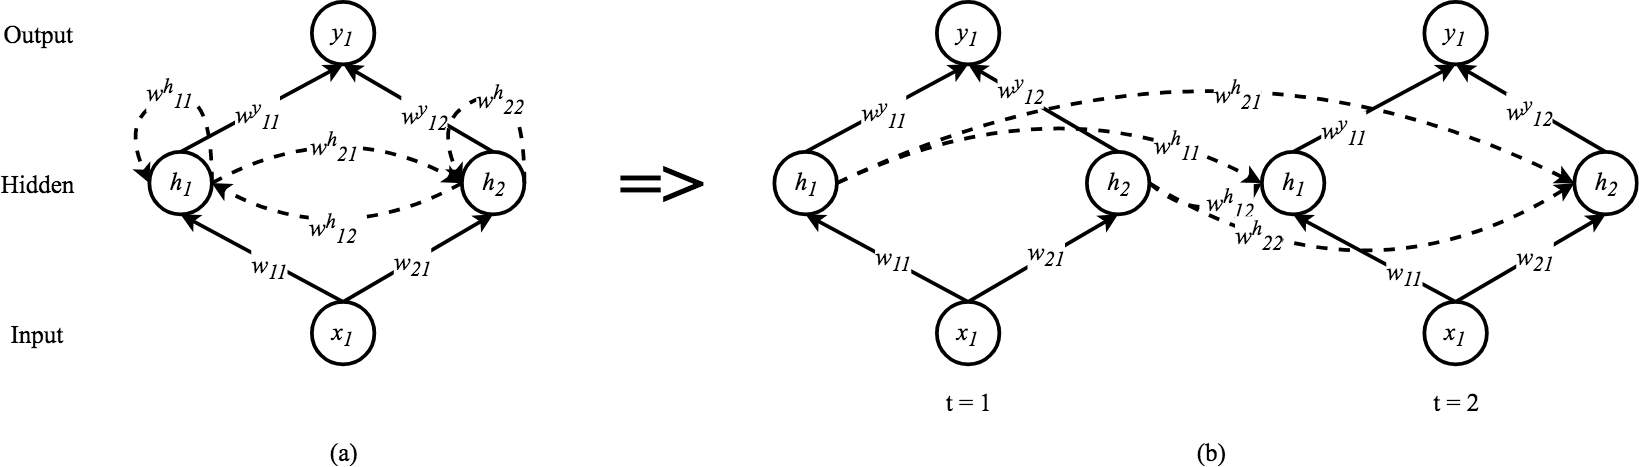
\includegraphics[width=0.8\textwidth]{recurrent-neural-network}
\caption{A recurrent neural network with one hidden layer consisting of two units (a). The same neural network in (a) that is unfolded into two time steps (b).}
\label{fig:recurrent-neural-network}
\end{figure}
%%%%%%%%%%%%%%%%%%%%%%

\subsubsection{Long Short-Term Memory Units}
RNNs encounter difficulties when modeling arbitrary long sequences. When training RNNs on longer sequences the internal weights become too small to be able to capture any context. This is know as the vanishing gradient problem and long short-term memory units (LSTMs) were introduced to overcome this problem\cite{DBLP:journals/corr/Lipton15}. LSTMs employ gating elements that select which parts of the context the unit should "remember" and the parts that it should "forget"\cite{LSTM}.
The use of LSTM in RNN architecture allows long term dependencies in data to be remembered within the model \citep{Graves2013a}, a feature that can be exploited to predict the next value of the sequence. If the predicted value is equal to or within a reasonable range of the observed value, the observed value can be assumed to be valid. The observed value is missing or fails an outlier test, the predicted value replaces the missing value and becomes part of the input to the next sequence test.

\chapter{Model Selection and Evaluations Metrics :}\label{descriptors}

\section{model selection}\label{variance_bias}
Model selection is the process of choosing between different machine learning approaches,  or choosing between different hyperparameters or sets of features for the same machine learning approach  like in LSTM  finding the right look back parameter, and the number of layers, nodes.
The choice of the actual machine learning algorithm is less important than we'd think  there may be a "best" algorithm for a particular problem, but often its performance is not much better than other well performing approaches for that problem.

There may be certain qualities we look for in an model:
\begin{itemize}
\item Interpretable   can we see or understand why the model is making the decisions it makes?
\item Accurate
\item Fast (to train and test)
\item Scalable (it can be applied to a large dataset)
\end{itemize}
Though there are generally trade offs among these qualities.\\in order to select a model from other models, we usually use one of the following approaches.\\\textbf{A Typical approach } is to take your data and split it randomly into a training set and a test set (e.g. a 70\%/30\% split). Then you train your model on the training set and see how it performs on the test set.\\The problem with this approach is that it results in an overly optimistic estimation of generalization if we tune our model's parameters with it,  so what we want to do instead is splitting the data is to not split it only into training and testing sets, but to also include a validation set. A typical ratio is 60\% training, 20\% validation, 20\% testing.

This way we can measure validation error instead of just measuring the test error .
We can use these errors   to identify what kind of problem we have if our model isn't performing well:

\begin{itemize}
\item If our training error is large and our validation/test set error is large, then we have a high bias (underfitting) problem.
\item If our training error is small and our validation/test set error is large, then we have a high variance (overfitting) problem.
\end{itemize}
As the figure \ref{fig:bias} explains : 
\begin{figure}[H]
\centering
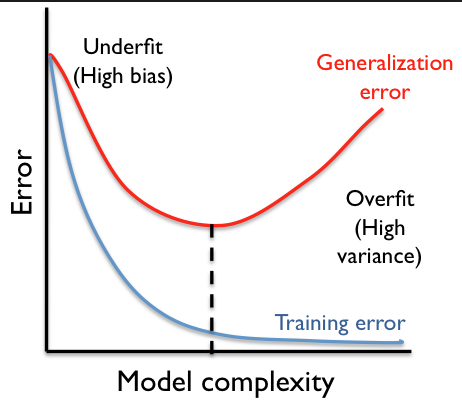
\includegraphics[width=0.38\textwidth]{img/model.png}
\caption{ bias / variance Tradeoff}
\label{fig:bias}
\end{figure}
Some ways of evaluating a model's performance on (some of)  known data are for \textbf{validation set } to pick  the best model you can possibly get :
\begin{itemize}
\item Hold out (just set aside some portion of the data for validation; this is less reliable if the amount of data is small such that the held out portion is very small) 
\item K-fold cross-validation (better than hold out for small datasets) for better visualization  check figure \ref{fig:cross}
%
\begin{itemize}
\item The training set is divided into k folds
\item Iteratively take k-1 folds for training and validate on the remaining fold
\item Average the results
\item There is also "leave-one-out" cross-validation which is k-fold cross-validation where k=n (n is the number of data points)
\end{itemize}
%
%
\begin{figure}[H]
\centering
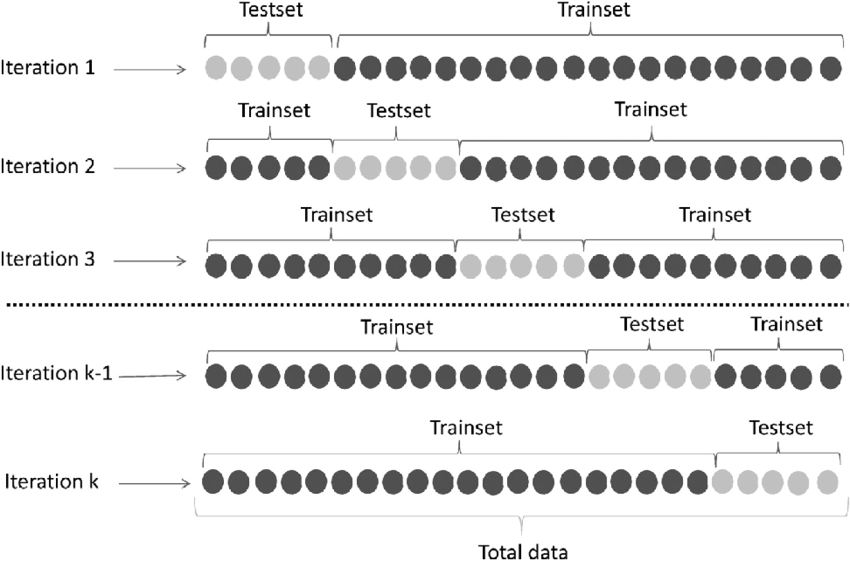
\includegraphics[scale=0.9]{img/cross.png}
\caption{K-cross validation }
\label{fig:cross}
\end{figure}
%
\item Bootstrapping : 
\begin{itemize}
\item New datasets are generated by sampling with replacement (uniformly at random) from the original dataset
\item Then train on the bootstrapped dataset and validate on the unselected data
\end{itemize}
\end{itemize}
%
\subsection{Evaluating classification models}\label{eva}
Every model comes with parameters that can modify the model's behavior and performance, evaluation of the model  often comes in the form of a confusion matrix \ref{confu}.
% Please add the following required packages to your document preamble:

% Please add the following required packages to your document preamble:
% \usepackage{multirow}
\begin{table}[]
\centering
\caption{Confusion matrix}
\label{confu}
\begin{tabular}{lllclll}
\cline{3-4}
                                                                                                        & \multicolumn{1}{l|}{}           & \multicolumn{2}{l|}{\textbf{Predicted Class}}                                                                                                                                                            &                               &  &  \\ \cline{3-4}
                                                                                                        & \multicolumn{1}{l|}{}           & \multicolumn{1}{l|}{\textbf{P}}                                                                    & \multicolumn{1}{l|}{\textbf{N}}                                                                     &                               &  &  \\ \cline{1-4}
\multicolumn{1}{|l|}{\multirow{2}{*}{\textbf{\begin{tabular}[c]{@{}l@{}}Actual \\ Class\end{tabular}}}} & \multicolumn{1}{l|}{\textbf{P}} & \multicolumn{1}{l|}{\textbf{\begin{tabular}[c]{@{}l@{}}True Positives\\        (TP)\end{tabular}}} & \multicolumn{1}{l|}{\textbf{\begin{tabular}[c]{@{}l@{}}False Negatives\\        (FN)\end{tabular}}} & \multicolumn{1}{c}{\textbf{}} &  &  \\ \cline{2-4}
\multicolumn{1}{|l|}{}                                                                                  & \multicolumn{1}{l|}{\textbf{N}} & \multicolumn{1}{c|}{\textbf{\begin{tabular}[c]{@{}c@{}}False Positives\\ (FP)\end{tabular}}}       & \multicolumn{1}{c|}{\textbf{\begin{tabular}[c]{@{}c@{}}True Negatives\\ (TN)\end{tabular}}}         & \textbf{}                     &  &  \\ \cline{1-4}
                                                                                                        &                                 & \multicolumn{1}{c}{\textbf{}}                                                                      & \textbf{}                                                                                           & \multicolumn{1}{c}{\textbf{}} &  &  \\
                                                                                                        &                                 & \multicolumn{1}{c}{\textbf{}}                                                                      & \textbf{}                                                                                           & \multicolumn{1}{c}{\textbf{}} &  & 
\end{tabular}
\end{table}


The core values are:
\begin{itemize}
\item True positives (TP): samples classified as positive which were labeled positive
\item True negatives (TN): samples classified as negative which were labeled negative
\item False positives (FP): samples classified as positive which were labeled negative
\item False negatives (FN): samples classified as negative which were labeled positive
\end{itemize}

here is some important quantities we need to know in order to evaluate a model :
\begin{itemize}
\item Recall  also known as True Positive Rate (TPR): $ \frac{TP}{TP+FN}$ 
\item False Positive Rate (FPR): $\frac{TN}{TN+FP}$
\item Positive predictive value:  $\frac{TP}{TP+FP}$ 
\item Negative predictive value: $\frac{TN}{TN+FN}$
\item Precision: How many of the predicted positive samples are correctly predicted   $\frac{\text{TP}}{\text{TP} + \text{FP}}$

\item Accuracy : $\frac{TP+TN}{TP+FP+TN+FN}$

\item The F-score is often introduced as harmonic mean of precision and recall.

$F$-$score= \frac{\text{2} \cdot \text{Precision } \cdot \text{ Recall} }{ \text{Precision} + \text{ Recall}}$
\end{itemize}


\subsection{Performance measures}
Final parameter selection and performance were measured by Mean Absolute Error (MAE) given by 
%
\begin{equation}
\label{eq:MAE}
MAE = \frac{1}{n}\sum^{n}_{i=1} \left | y_{obs_{i}}- y_{pred_{i}} \right |
\end{equation}
%
and Root Mean Square Error given by
%
\begin{equation}
\label{eq:RMSE}
RMSE = \sqrt{\frac{1}{n}\sum^{n}_{i=1} \left ( y_{obs_{i}}- y_{pred_{i}} \right )^{2}}
\end{equation}
MAE and RMSE are widely used measures of continuous variables with RMSE criticized for over-biasing towards large errors \cite{Chai2014Willmott2005}. Both metrics were calculated for comparison; however MAE is used more often for descriptive analytics.
\subsubsection{Area under the ROC curve (ROC AUC)}
Receiver Operating Characteristics  ( ROC) is a method that visualizes, organizes and selects models based on  their performance,  this method is for binary classification, but we can adapt it to multi-classification problem  using "OneVsAll" approach, it basically  visualizes the performance of our classifier through all the thresholds, whereas accuracy and F-score  metrics, etc, judge the performance based on particular threshold (usually  0.5) above this cut-off one label is assigned, and below it the other label is assigned. But  looking at all thresholds at once, can give a clear and more honest image of the real performance of our classifier,  since  some models may work best with a different threshold and data sometimes can be biased,   that's when  a dataset has way more or way less of the positive class than there are of the negative class. This imbalance in data can give deceptive and false results if we used accuracy as a metric, to clear the idea more let's say we have a dataset of 100 training example in which it  has 99 example positive and 1 negative example.  The accuracy here can be very deceptive with a value of 99\% so accuracy can't tell much here, the F$\textbf{-}$score can take  into consideration these kind of unbalanced data,  by considering  the true \textbf{positive } rate and the true \textbf{predictive} value  but  it does  not consider all the thresholds of the classifier. However  ROC  is insensitive to bias data ( unbalanced data ) and can run over all thresholds and plots, the  true vs false positive rates, varying the threshold can give us pair of (FPR,TPR) \ref{fig:bias2}.
\begin{figure}[H]
\centering
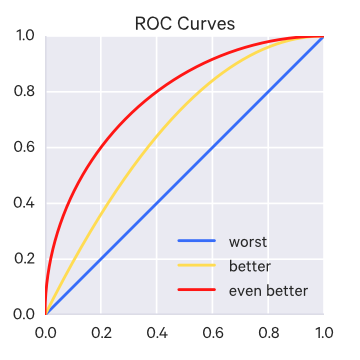
\includegraphics[width=0.45\textwidth]{img/roc.jpg}
\caption{ ROC curve }
\label{fig:bias2}
\end{figure}
The area under the curve (AUC) is used to quantify how good the classifier is. The AUC is in fact  the probability that a classifier will rank a randomly chosen positive instance higher than a randomly chosen negative one, (assuming 'positive' ranks higher than 'negative'). Generally, an AUC of above 0.8 is considered "good", an AUC of 0.5 (a straight line) is equivalent to random guessing.


\section{Conclusion:}

In this chapter we have presented in detail some of the most popular  methods for selecting  a model using K-fold cross validation, and their astonishing role in maximizing the performance of a classifier by choosing the optimal hyperparameters of a model.
Finally we reviewed  how to  assess the performance of a fully trained classifier using area under ROC curve ( ROC AUC ).
In the next chapter we will finally take a look on the techniques used for imputation, and we will discuss multiple results.


\chapter{Methodology} \label{ML}


\subsection{Context Of Imputation in Real World Data :}\label{contextofimp}
 Continuous time series data is collected by different stations and systems, the missing data can be produced due to the transfer problems or natural disaster that can damage devices (sensors), or any external factor, furthermore this leads us to the question “ How can we impute data that does not exist ? ”, One solution is imputing  data from the nearest neighbor of the damaged sensor, this solution is very dangerous, we will  consider the following example to clear the problem more.
let S = {s1 s2 s3 s4 } be a set of sensors that is distributed as following s1 is a sensor  that measure the temperature of soil, s2 is a sensor of temperature but in 2km away from S1 in a certain direction but its height is about 10 m above the level of s1 height, s3  is 5km away from s1 that measure also temperature of soil,  s4  is 3km away from s1  and  measures Humidity.

Now in the hypothesis of imputing data of sensor s1  using nearest neighbor approach if wrong, because the nearest  sensor is s2  that has the same physical property (temperature) is measuring  temperature in 10 m which is very different from the soil temperature, in this case it would be logical to choose s3 even if it is far from s2 . or a combination of s3 and s4 even if this last measure different physical quantity (humidity) but it is correlated to temperature, and it can help imputing missing values.

A better solution that we would like to build is a system that is able to choose the right combination of sensors to impute data of a damaged sensor, this system should be able to learn the right correlations needed to impute each sensor, which leads us to using Deep learning models like Recurrent Neural Networks (RNN) and its various architecture, hoping this model will learns the right inter-correlations and predict the right missing values.

\subsection{Data used}
the  data used in this project, is a real world traffic data, it was collected from  monitoring stations located between Nancy and  Metz  A31  road ''La Direction Interdépartementale des Routes Est (DIR Est) '', the idea of the project is to study  how  a set of speed limits displays that change in time dependent on a lot of factors, would actually reduce the traffic congestion.
and for that they took measures of Speed and Flow rate, of course there other Spatial features like the section of sensor (refered to as station), there are also 2 sens and some times 3 sens in a road, and other features that allocate spatially where sensors are.
but one thing let their Data scientist, struggle to have a conclusion was Missing Data values.


\begin{figure}[H]
\centering
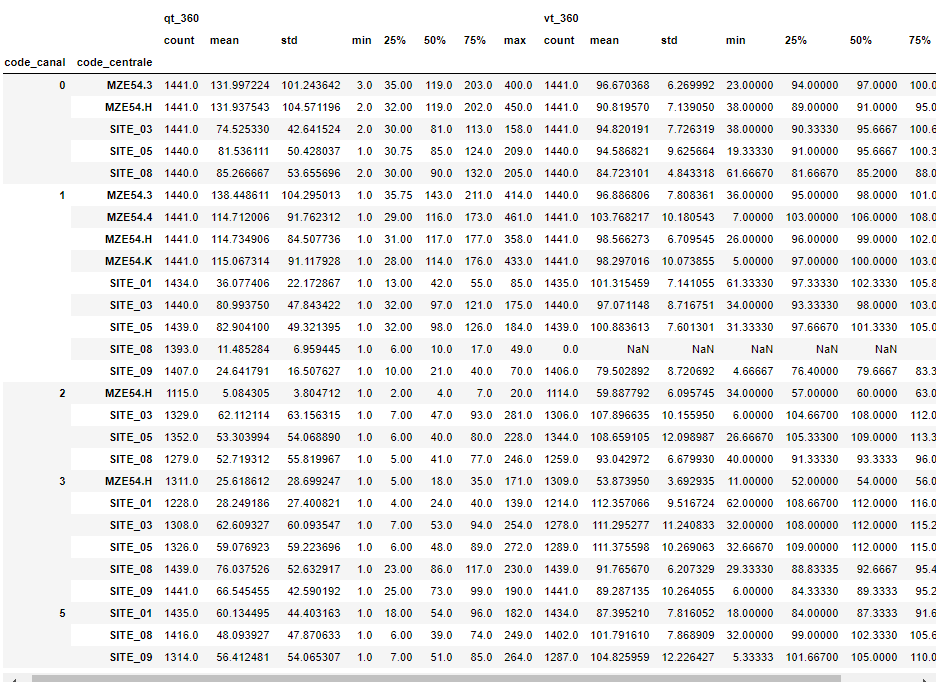
\includegraphics[scale=.55]{img/grouped_data_descriptives.png} 
\caption{traffic Dataset descriptive statistics}
\label{fig:score}
\end{figure}


\subsection{classical methods :}

the distribution of missing data is not following any pattern, which favor the hypothesis of being Missing at random, which is the case of 90\% in real world data.

%
\begin{figure}[H]
\centering
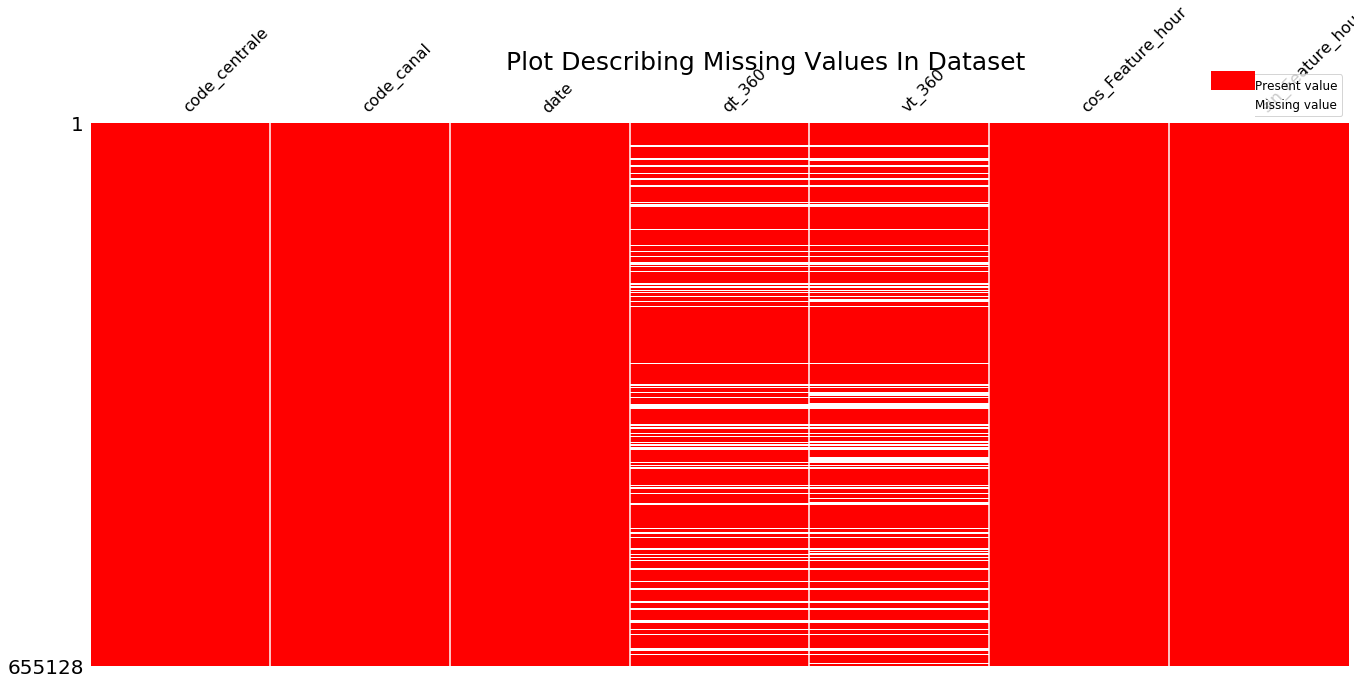
\includegraphics[width=.9\textwidth]{img/missing_values_distributation.png} 
\caption{Missing data distribution of all features in Dataset}
\label{fig:presteps}
\end{figure}
%

the naive solution is to impute (fill) missing values using mean values of each feature. which seems reasonable estimate except that this is not safe to use even if your missing observation are completely at random. However, clearly this is not the case we are dealing with, the mean  method may lead to inconsistent bias. 

The figure below shows the imputation  using Mean and Standard Deviation,  here we have a gap of 3 days, No additional information was added, the mean only make  the size of time serie bigger, this leads to an underestimate of the errors [\ref{}].
%
\begin{figure}[H]
\centering
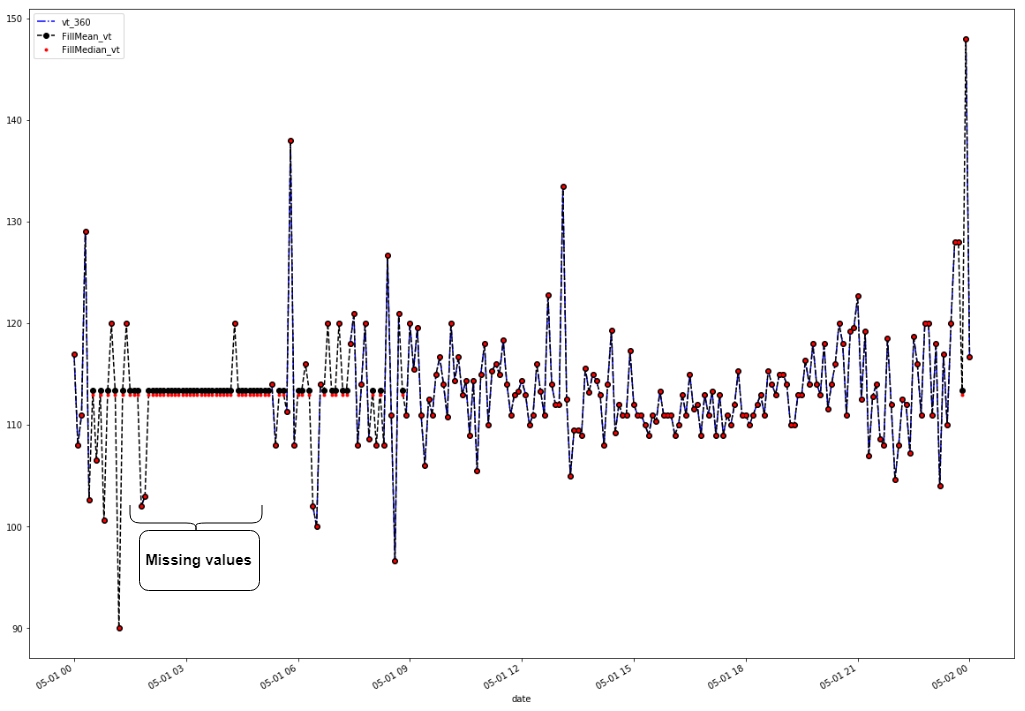
\includegraphics[scale=.4]{img/mean_median.png} 
\caption{Mean and standard Deviation imputation}
\label{fig:presteps}
\end{figure}
%
on the other hand one may try only to interpolate using linear interpolation or even add more polynomial degrees, and quantify the error made by different interpolation techniques.

\begin{figure}[H]
\centering
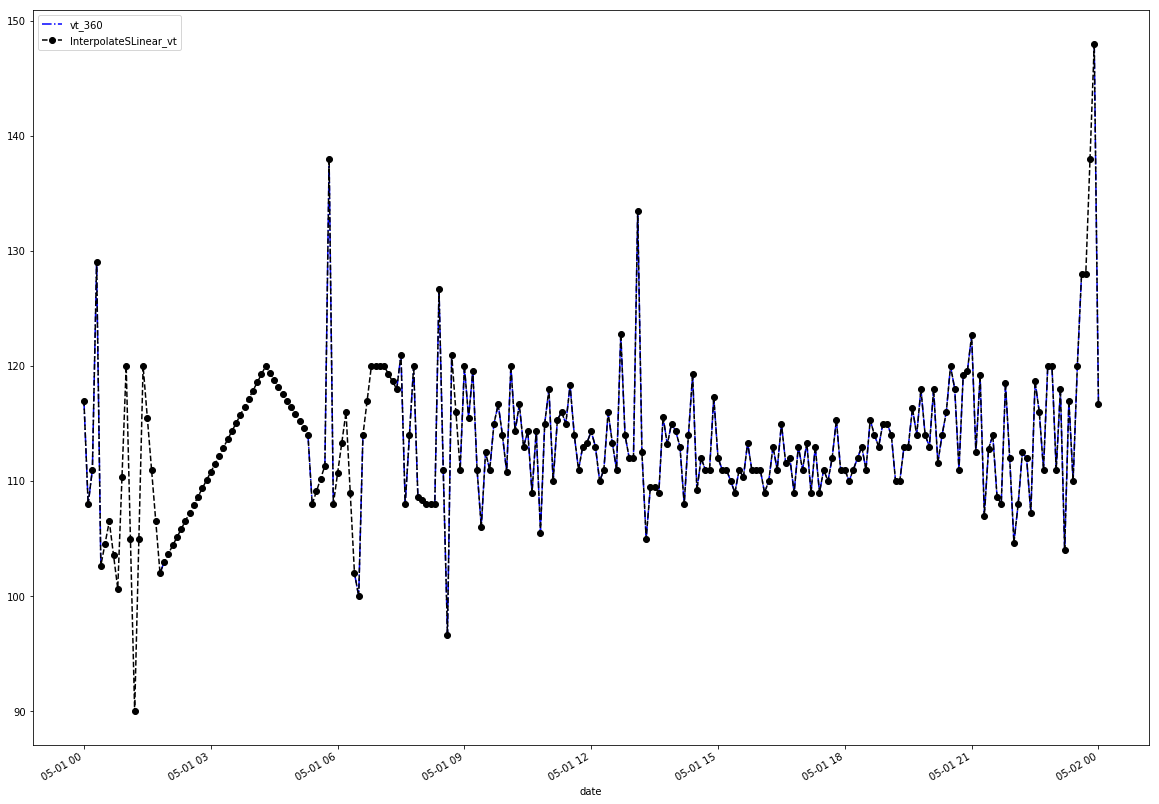
\includegraphics[scale=.33]{img/linear.png} 
\caption{Imputation using Linear Interpolation }
\label{fig:presteps}
\end{figure}


%
% \begin{figure}[H]
% \centering
% 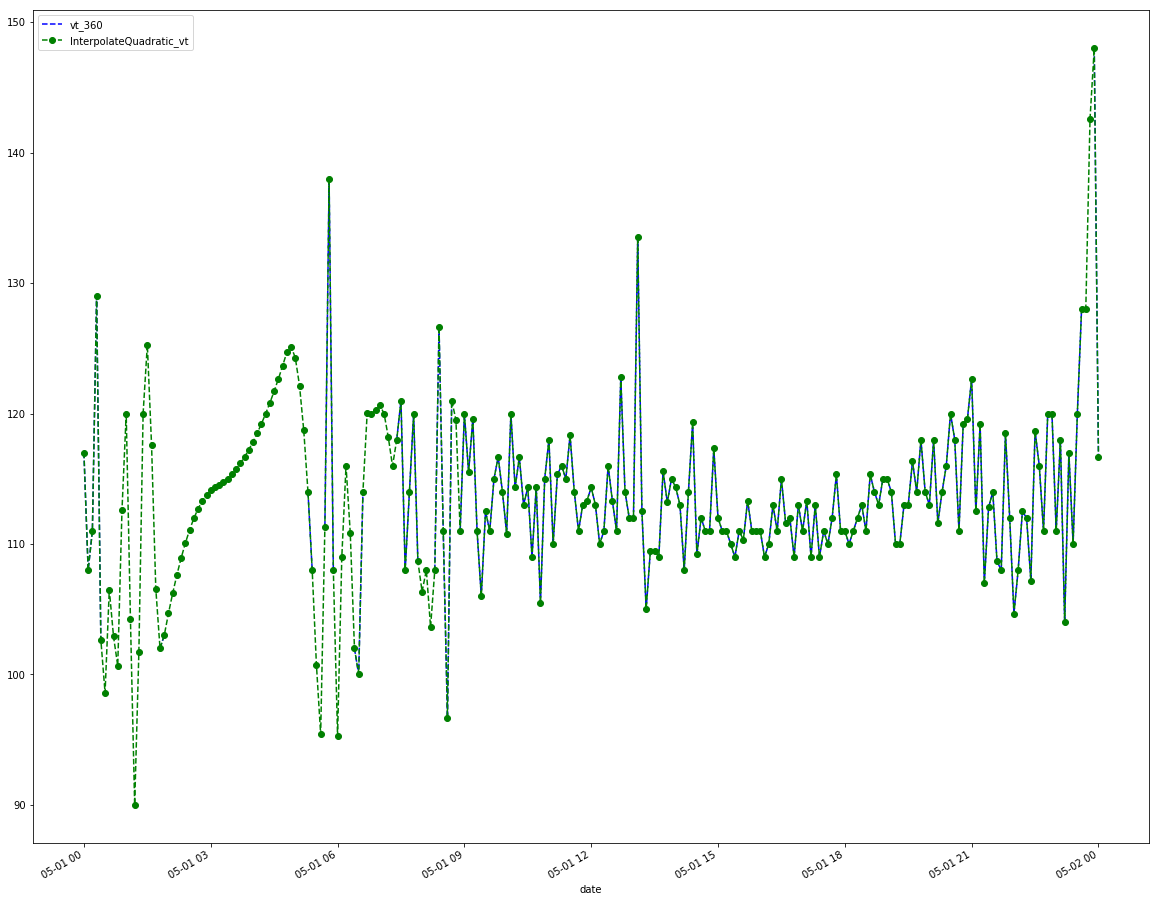
\includegraphics[width=.75\textwidth]{img/quadratic.png} 
% \caption{Imputation using Quadratic Interpolation}
% \label{fig:presteps}
% \end{figure}

% %
% \begin{figure}[H]
% \centering
% 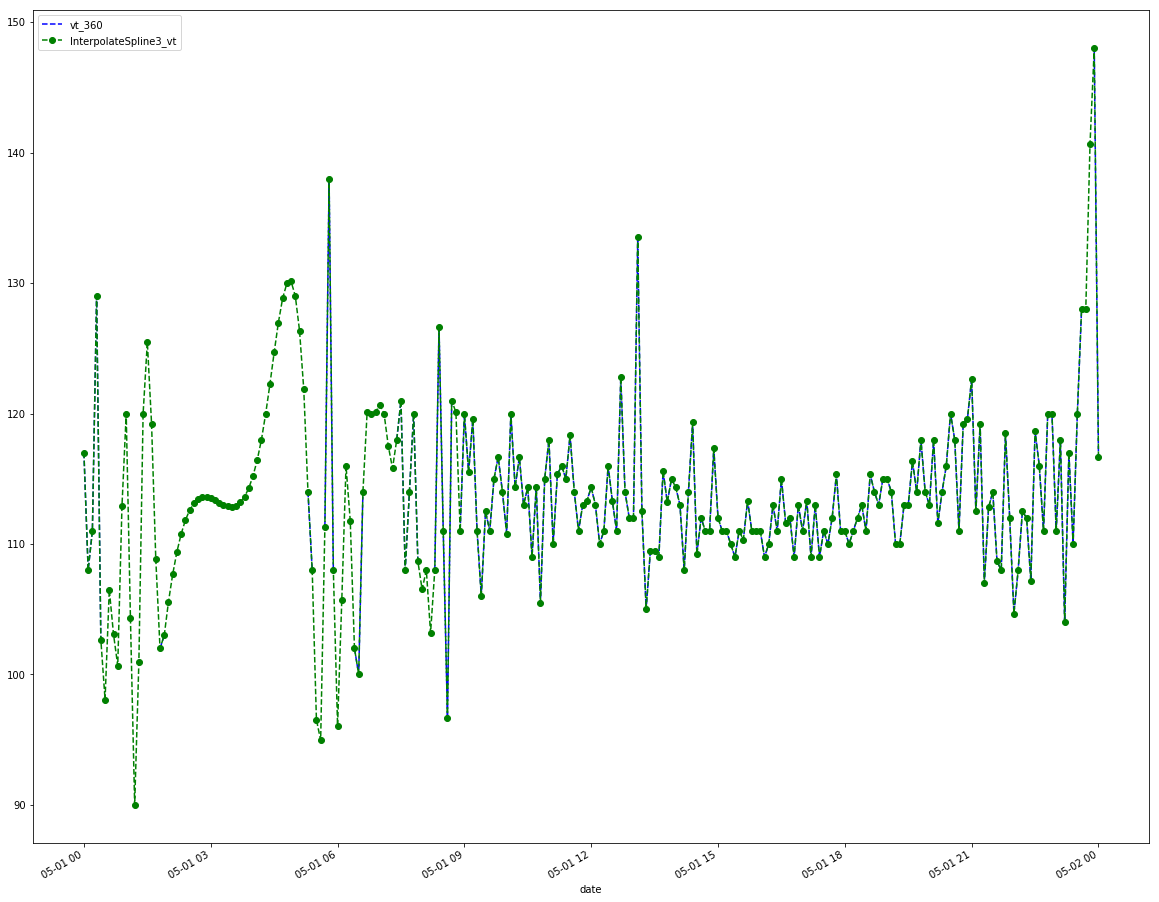
\includegraphics[width=.75\textwidth]{img/spline.png} 
% \caption{Spline interpolation for imputation}
% \label{fig:presteps}
% \end{figure}
%%

\begin{figure}[h]
\centering
\begin{minipage}{.49\linewidth}
    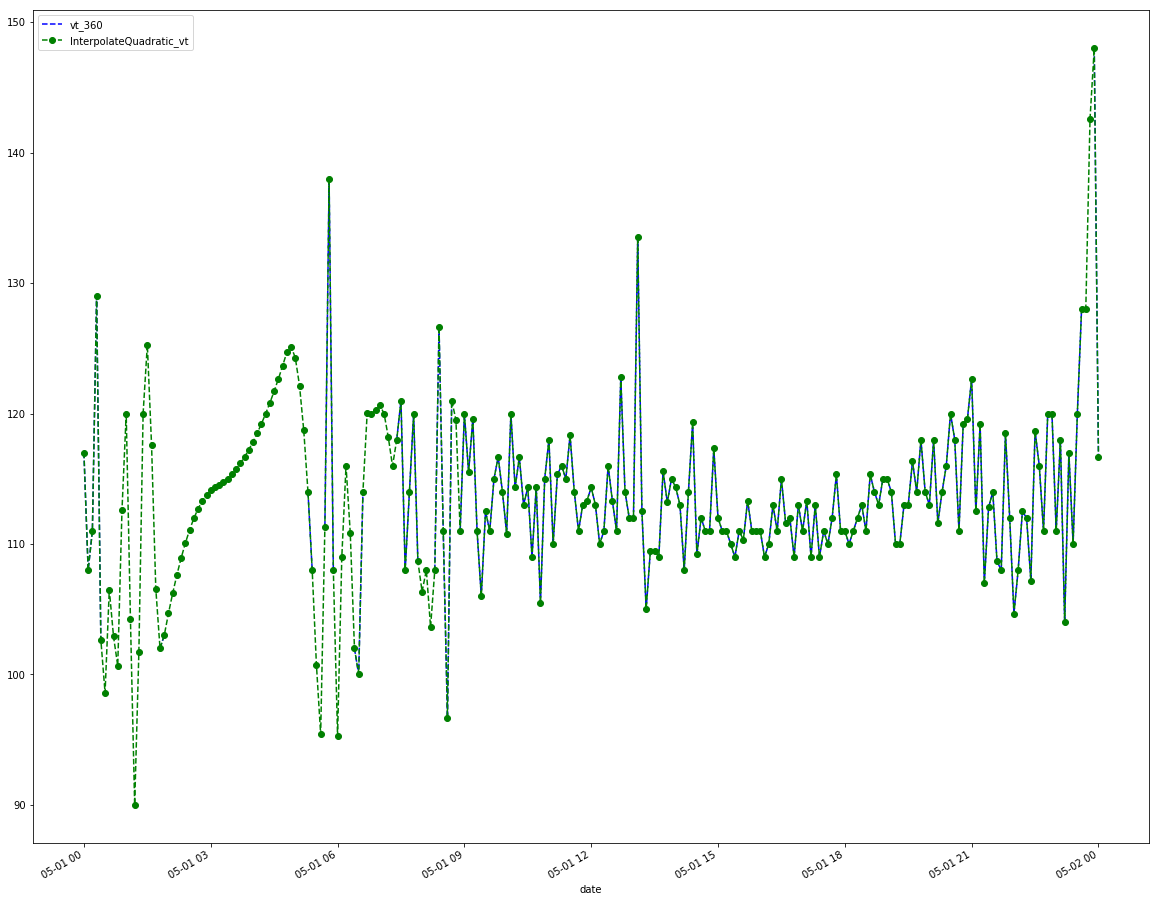
\includegraphics[width=.9\textwidth]{img/quadratic.png}    
    \caption{Quadratic Interpolation}
    \label{img1}
\end{minipage}
\hfill
\begin{minipage}{.49\linewidth}
    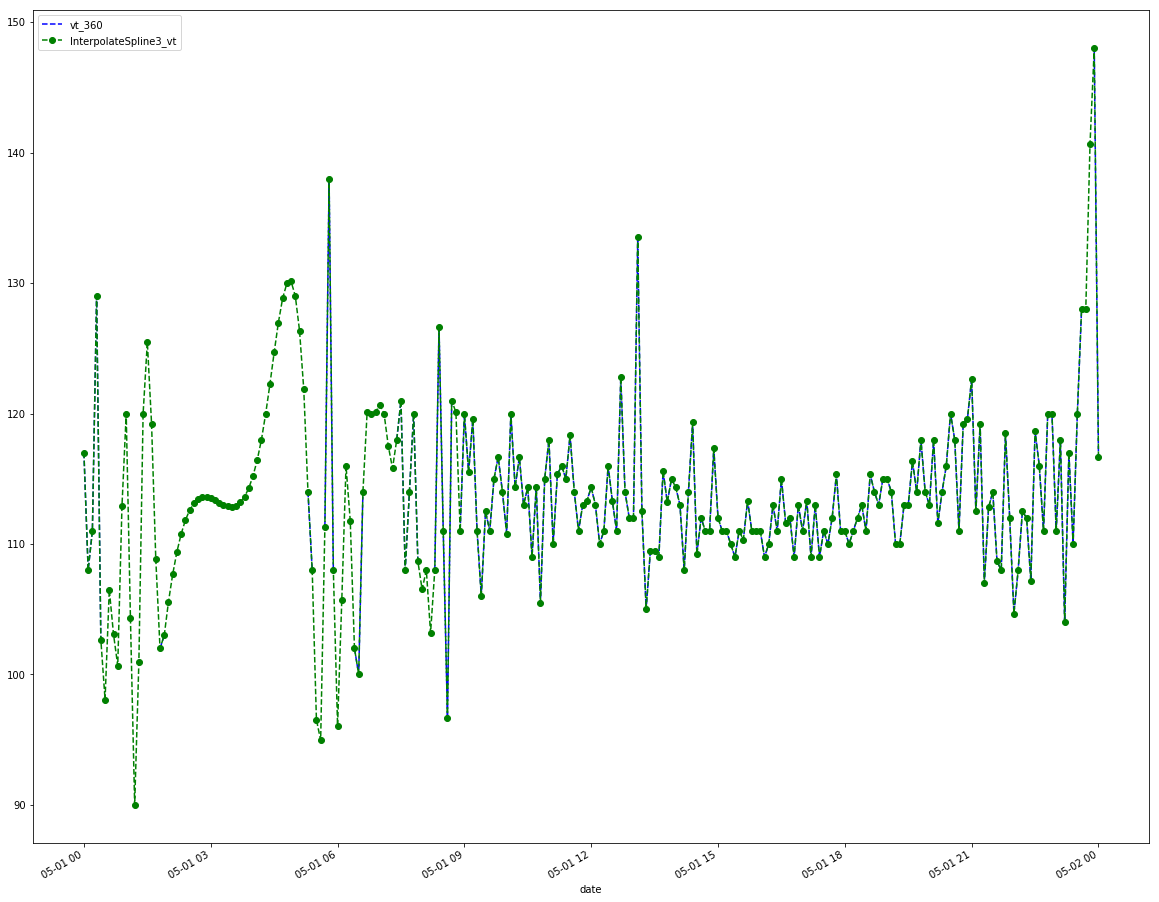
\includegraphics[width=.9\textwidth]{img/spline.png} 
    \caption{Spline interpolation for imputation}
    \label{img2}
\end{minipage}
\end{figure}


Scoring the results and see which is better, we can see from figure below [\ref{fig:score}], that both linear interpolation and interpolation Time is giving the minimum error compared to other methods.

\begin{wrapfigure}{!l}{0.35\textwidth}
\centering
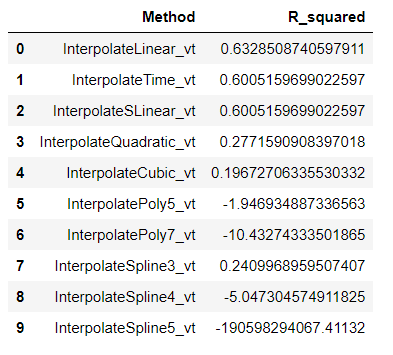
\includegraphics[width=.4\textwidth]{img/results_R.png} 
\caption{Missing data distribution of all features in Dataset}
\label{fig:score}
\end{wrapfigure}
we can see clearly how inefficient these methods are and can introduce bias data to work with later or train on.thus, these methods cannot be employed, as they are not  based on inter-variable correlations, neither they take the time dimension into account as a major feature in order to estimate missing values. For instance the interpolation methods tries to fit a “smooth curve” fitting the observed data and this way we approximate the missing values but with a really poor hypothesis that will need a lot of constraints to be true. Also it discards any relationships between the variables over time. Other methods that are usually used for times series predictions ( the autoregressive methods like ARIMA) can hold the answer for our problem.


\subsection{ ARIMA (Autoregressive Integrated Moving Average):}
as we already mention in state of the art ARIMA is a very famous method for forcasting in finance and Time Series Data,  
Box and Jenkins proposed a set of guidelines that can be followed when
selecting ARIMA models. This systematic procedure to designing ARIMA
models has made them highly popular (Hibon and Makridakis
\protect\hyperlink{ref-spyros1997}{1997}).  It consists of a four-stage iterative process in which:

\begin{enumerate}
    \item  the process is either transformed or
differenced to de-trend\ref{fig:detrend} and stabilise the variance of the data.
 

\begin{figure}[H]
\centering
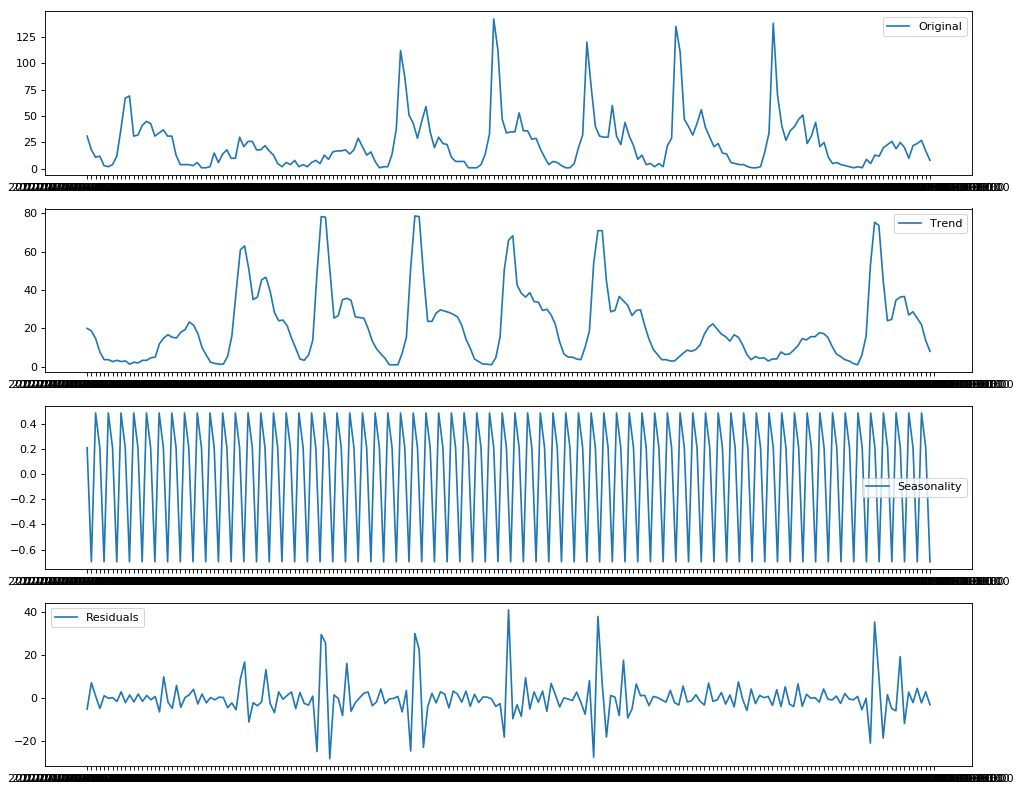
\includegraphics[scale=.4]{img/detreding.png} 
\caption{Remove trend and seasonality with decomposition }
\label{fig:detrend}
\end{figure}

\item the autocorrelation and partial autocorrelation plots are used to determine the order of p and q,
\item the parameters of the model are estimated,
\item a diagnostic check is performed to ensure that the residuals are a white noise process. If the residuals are not white noise steps 2-4 are repeated until a satisfactory model is identified. On the contrary, if the diagnostic check shows that the residuals are random then the developed model is the final model used for forecasting.
\end{enumerate}

It is important to keep in mind that regression techniques works on  observations that are independent of each other, we know that in time series all variables are time dependent, unless the time serie is Stationary we can not use any regression model.

To do so, we use  Dickey-Fuller test \ref{aaaa}, a statistical test with the null hypothesis that the time series is non-stationary. If the test results in the test statistic significantly less than the critical values, we can reject the null hypothesis in favor of time series stationarity.

as we may see in the figure below \ref{fig:duckeytest} our time serie is stationary :

\begin{figure}[H]
\centering
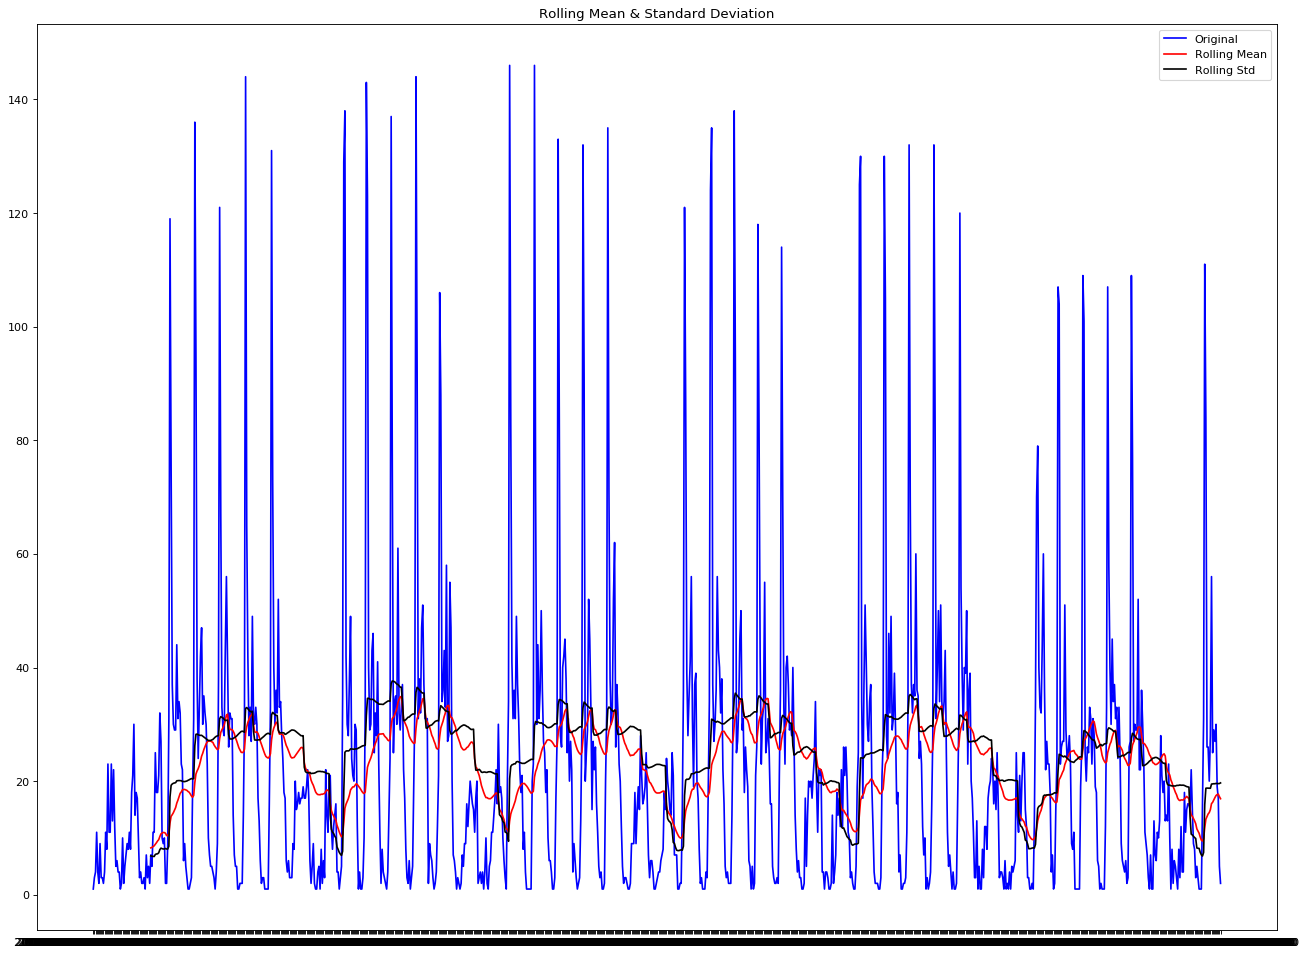
\includegraphics[scale=.35]{img/duckeyTest.png} 
\caption{imputation using Linear Interpolation }
\label{fig:duckeytest}
\end{figure}

Results of Dickey-Fuller Test:
\begin{wraptable}{!}{70mm}

\begin{tabular}{lllll}
\cline{1-2}
\multicolumn{1}{|l|}{\begin{tabular}[c]{@{}l@{}}Test Statistic                  \\ p-value                          \\ \#Lags Used                      \\ Number of Observations Used   \\ Critical Value (1\%)             \\ Critical Value (5\%)             \\ Critical Value (10\%)\end{tabular}} & \multicolumn{1}{l|}{\begin{tabular}[c]{@{}l@{}}-3.634985\\ 0.005126\\ 22.000000\\ 977.000000\\ -3.437061\\ -2.864503\\ -2.568348\end{tabular}} &  &  &  \\ \cline{1-2}
\end{tabular}
  \caption{Dickey-Fuller Test}

\end{wraptable}


The order of differencing is determined by using the KPSS test (Ruppert and Matteson \protect\hyperlink{ref-ruppert2015}{2015}). The KPSS test checks the null hypothesis of stationarity and sets d to zero if the null hypothesis is accepted, otherwise it iteratively increases d by 1 and tests the null hypothesis until it is accepted (Ruppert and Matteson \protect\hyperlink{ref-ruppert2015}{2015}). Once the order of
differencing has been determined, the order of p and q are chosen based on Akaike's Information Criterion (AIC) or the Bayesian Information Criterion (BIC) (Ruppert and Matteson \protect\hyperlink{ref-ruppert2015}{2015}).


Due to the large number of forecasts made, it is useful to have an
automatic procedure which is able to select the appropriate ARIMA model to fit the data. The \textbf{auto Arima} function in python, available also in R  is able to automatically choose the order of the parameters p, q and d.


\begin{figure}[H]
\centering
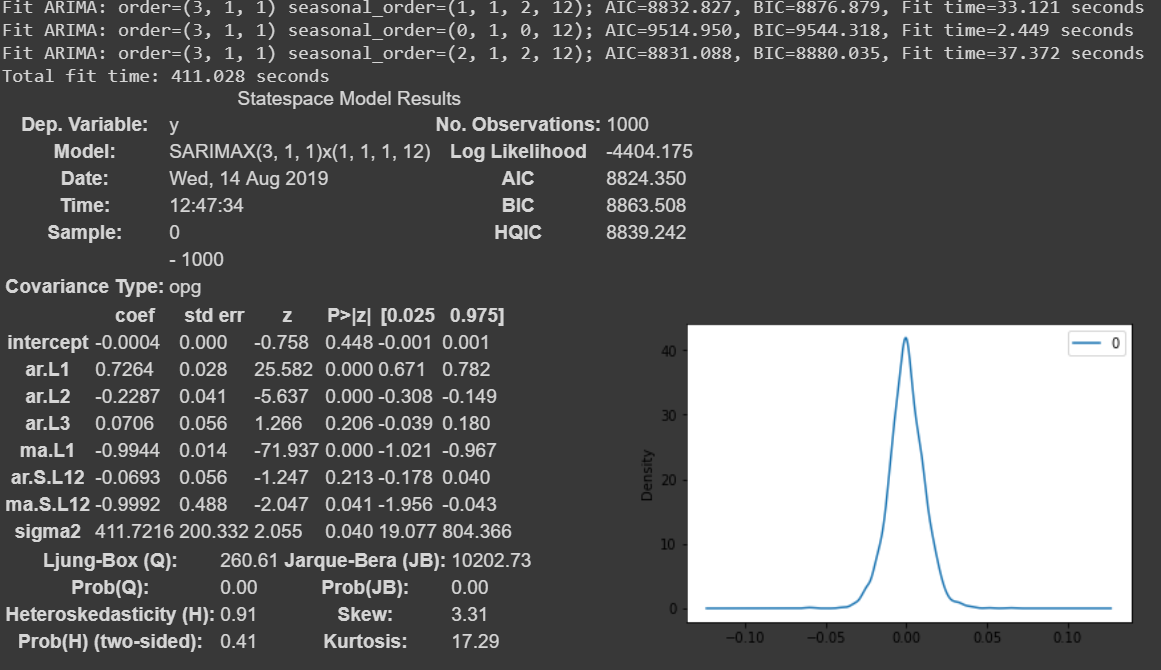
\includegraphics[scale=.6]{img/arima_degrees.PNG} 
\caption{Missing data distribution of all features in Dataset}
\label{fig:arima_degree}
\end{figure}

In order to validate the ARIMA model appropriateness is by performing residual analysis.

Print the results of the ARIMA model and plot the residuals as show in figure \ref{fig:arima_degree}. A density plot of the residual error values indicates a normal distribution centered around zero mean. Also, the residuals do not violate the assumptions of constant location and scale with most values in the range (-1,1).



in the next figures we can see the inference of  the best selected model with order=(3, 1, 1) and seasonal order=(2, 1, 2, 12). which scored an RMSE of 0.8 on the training data as in fig\ref{fig:trainig_arima}, we can forecast future event by just fitting the Arima model on the last  known data and have a forecasting as shown in figure \ref{fig:forcasting}.  


\begin{figure}[H]
\centering
\begin{minipage}{.49\linewidth}
    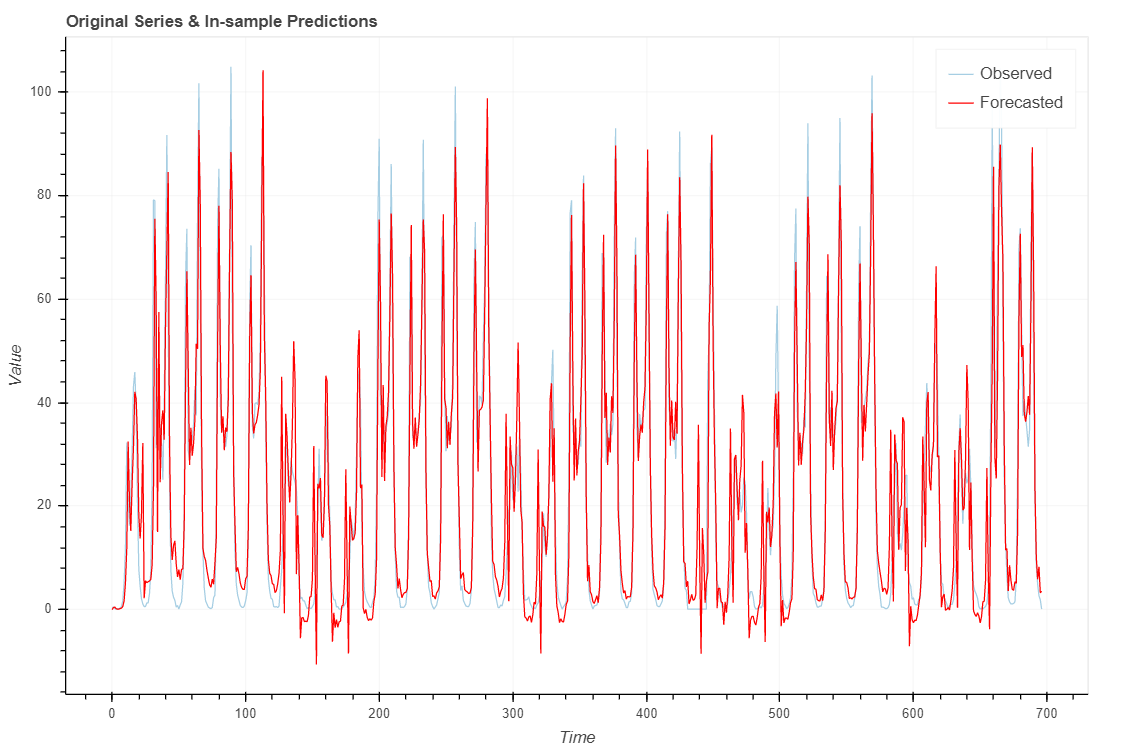
\includegraphics[width=.9\textwidth]{img/arima_training.png}    
    \caption{Arima prediction on training data}
    \label{fig:trainig_arima}
\end{minipage}
\hfill
\begin{minipage}{.49\linewidth}
    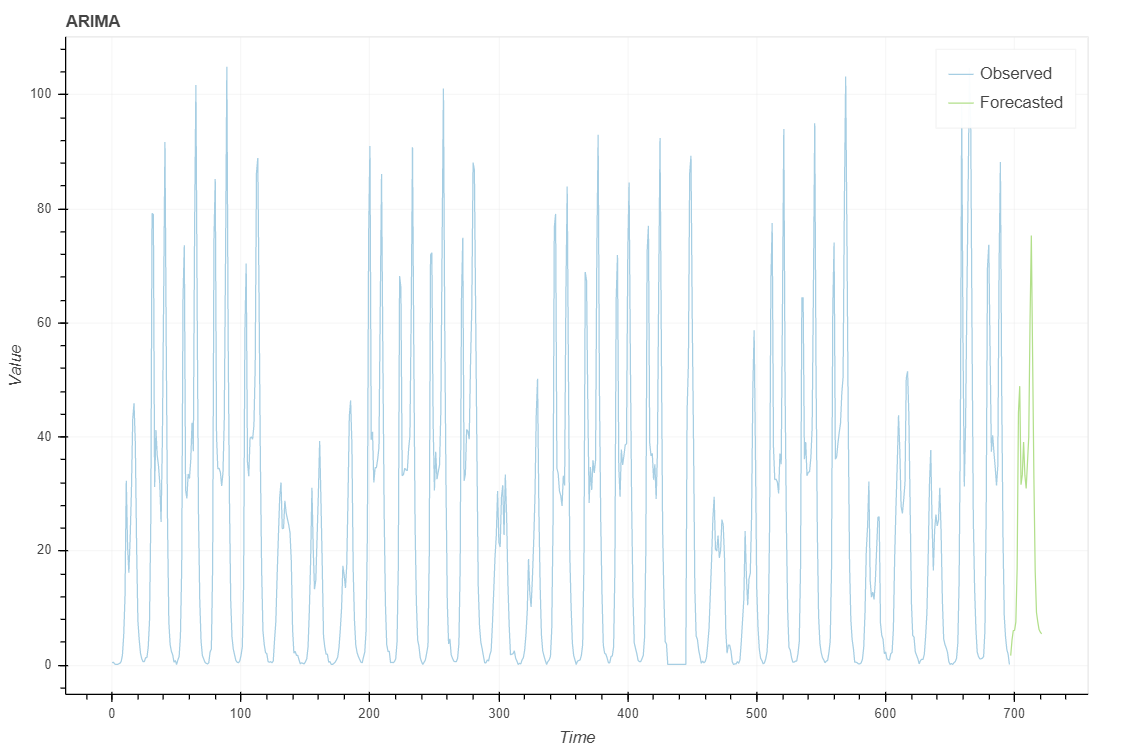
\includegraphics[width=.9\textwidth]{img/arima_forcasting.png} 
    \caption{Arima Forecasting}
    \label{fig:forcasting}
\end{minipage}
\end{figure}

now the idea as mentioned before is to go back to each gap and impute as if we want to infer and forecast the gap, The figure shown below shows the results obtained by imputing (filling), missing data by arima forecast.

\begin{figure}[H]
\centering
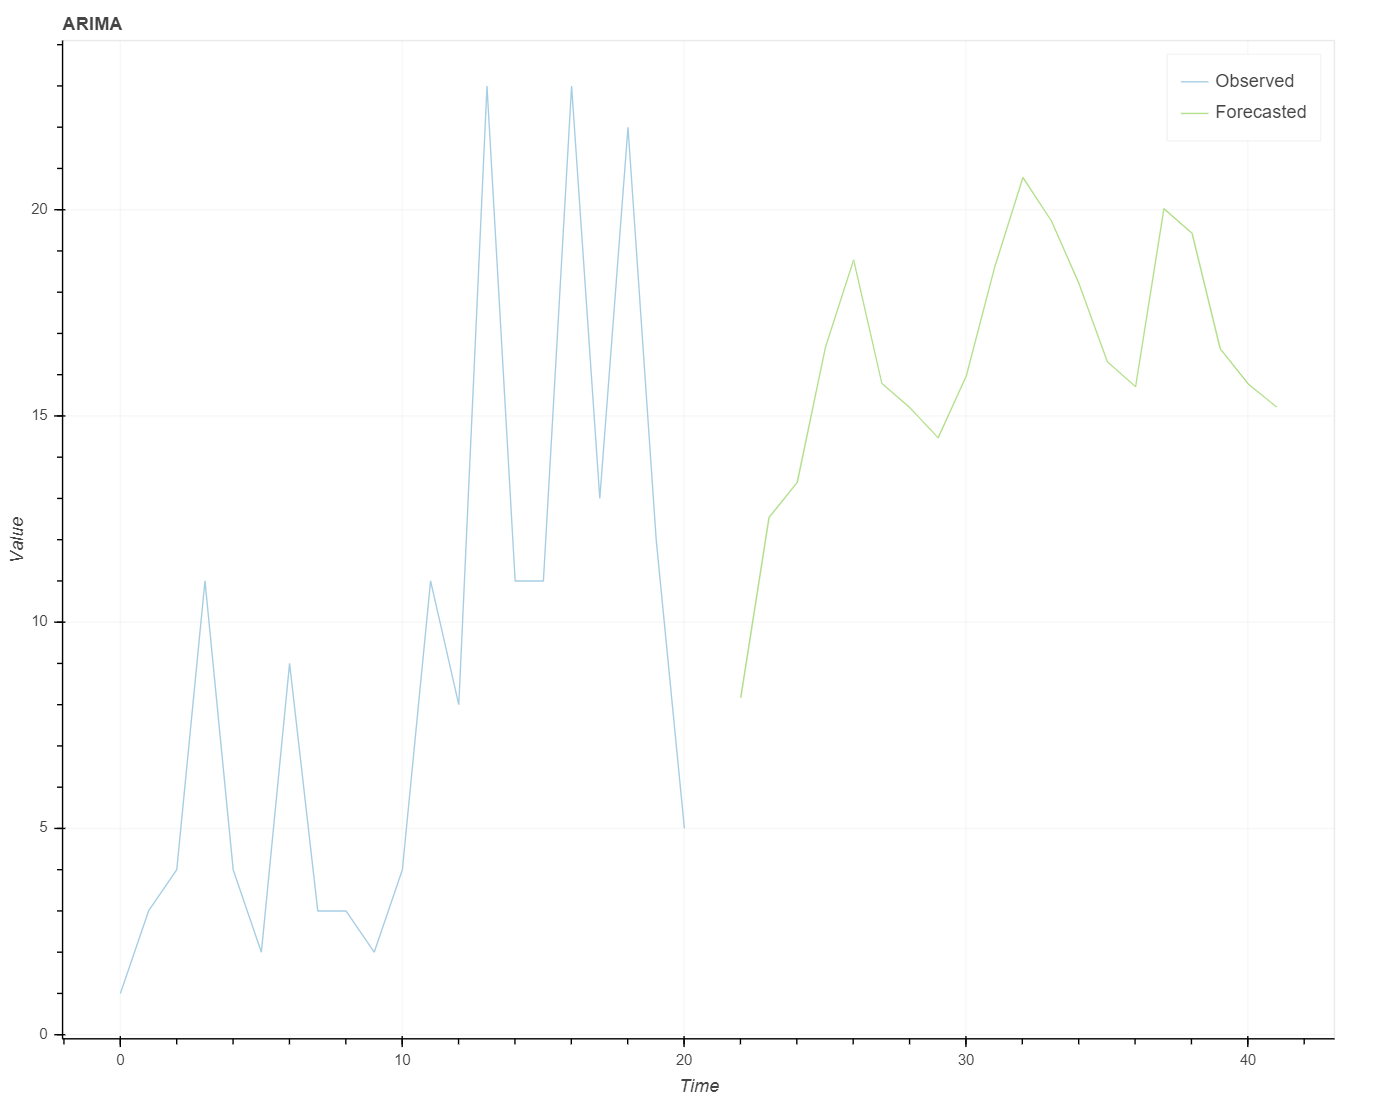
\includegraphics[scale=.2]{img/arima_imputation.png} 
\caption{Arima imputation}
\label{fig:arima_degree}
\end{figure}
often  in practice we use a kalman smoother to interpolate. 

Arima is good pratice for time series data and can give good result especially if you have small set of data, except that it eliminates the non-stationary parts in time series data and fit a parameterized stationary model, Also one of the biggest constraints why we can not proceed with ARIMA  is that we usually have multiple variables we need to use in order to impute  a damaged sensor, we need a model that can uses other's features to impute the missing data. 

As we have seen earlier the two models that can have a good modeling for time series and also  take into consideration all other features, are  Vector Auto-regressive (VAR) or Recurrent Neural Networks (RNN).

in  our Benchmarking, the VAR failed badly to fit even the Training Data, this is due to large amount of features. 

\begin{figure}[H]
\centering
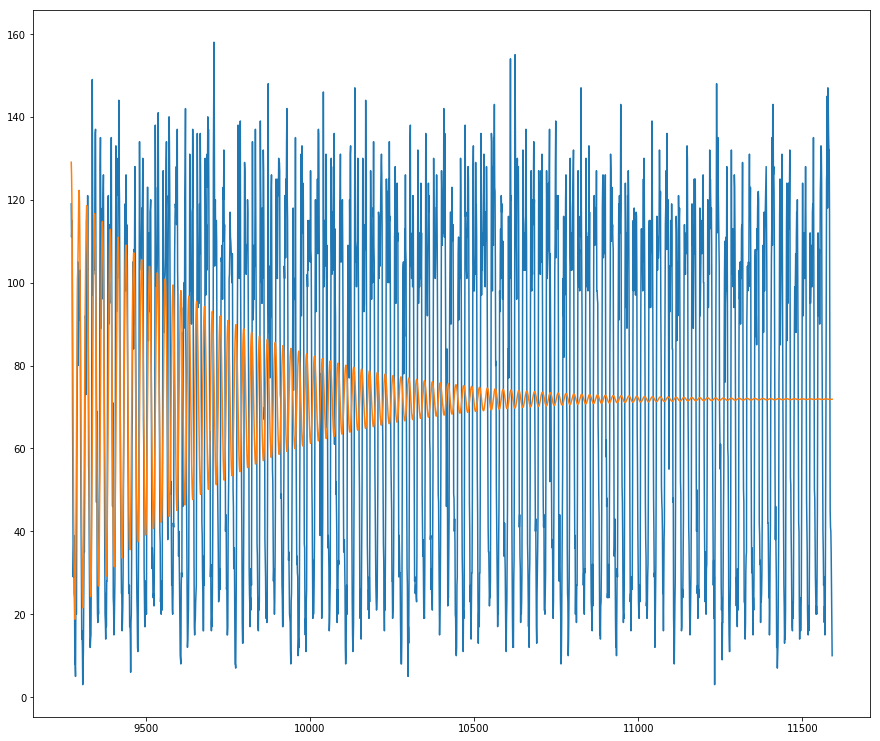
\includegraphics[scale=.2]{img/VAR.png} 
\caption{Vector Autoregressive VAR}
\label{fig:arima_degree}
\end{figure}

that left us with Deep learning approaches, Time series are sequential data whereas RNN is the state of the art to deal with sequential data.

\subsection{Building the RNN}
The RNN used was built on top of Keras API\cite{keras2015} with tensorflow  back-end. we used a variant of RNN called LSTM  that can even learn from larger dependencies, the coming list represents the specifications of the architecture used in this project:
\begin{itemize}
\item we used a the Many to one RNN architecture  uses a single output feed forward node as shown in figure \ref{fig:manyto_one}.

\begin{figure}[H]
\centering
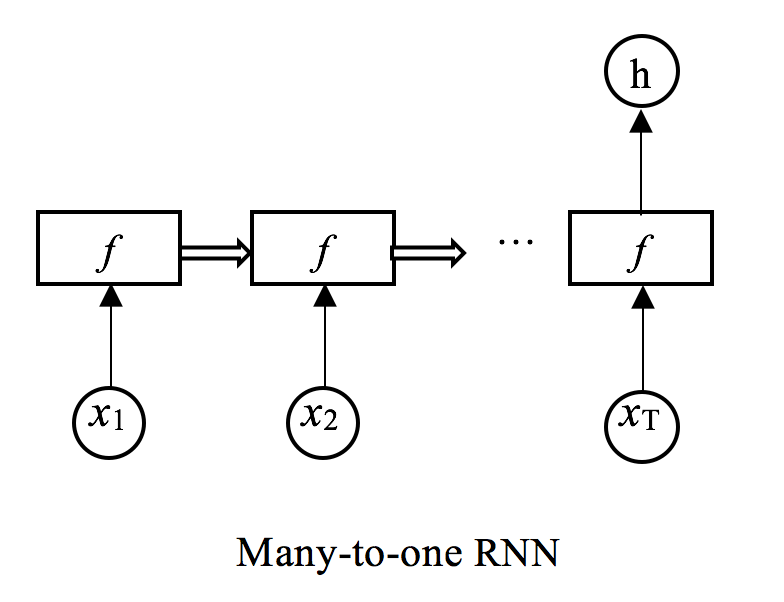
\includegraphics[scale=.3]{img/many_to_one.png} 
\caption{input as many time steps in the sequence, but the model produces only one output to predict the t+1 .}
\label{fig:manyto_one}
\end{figure}

    \item This architecture uses  $sigmoid$  as activation function for the output layers\ref{fig:lstmcell}.
    \item the activation function for the recurrent node was $tanh$ \ref{fig:lstmcell} .
\end{itemize}

\begin{figure}[H]
\centering
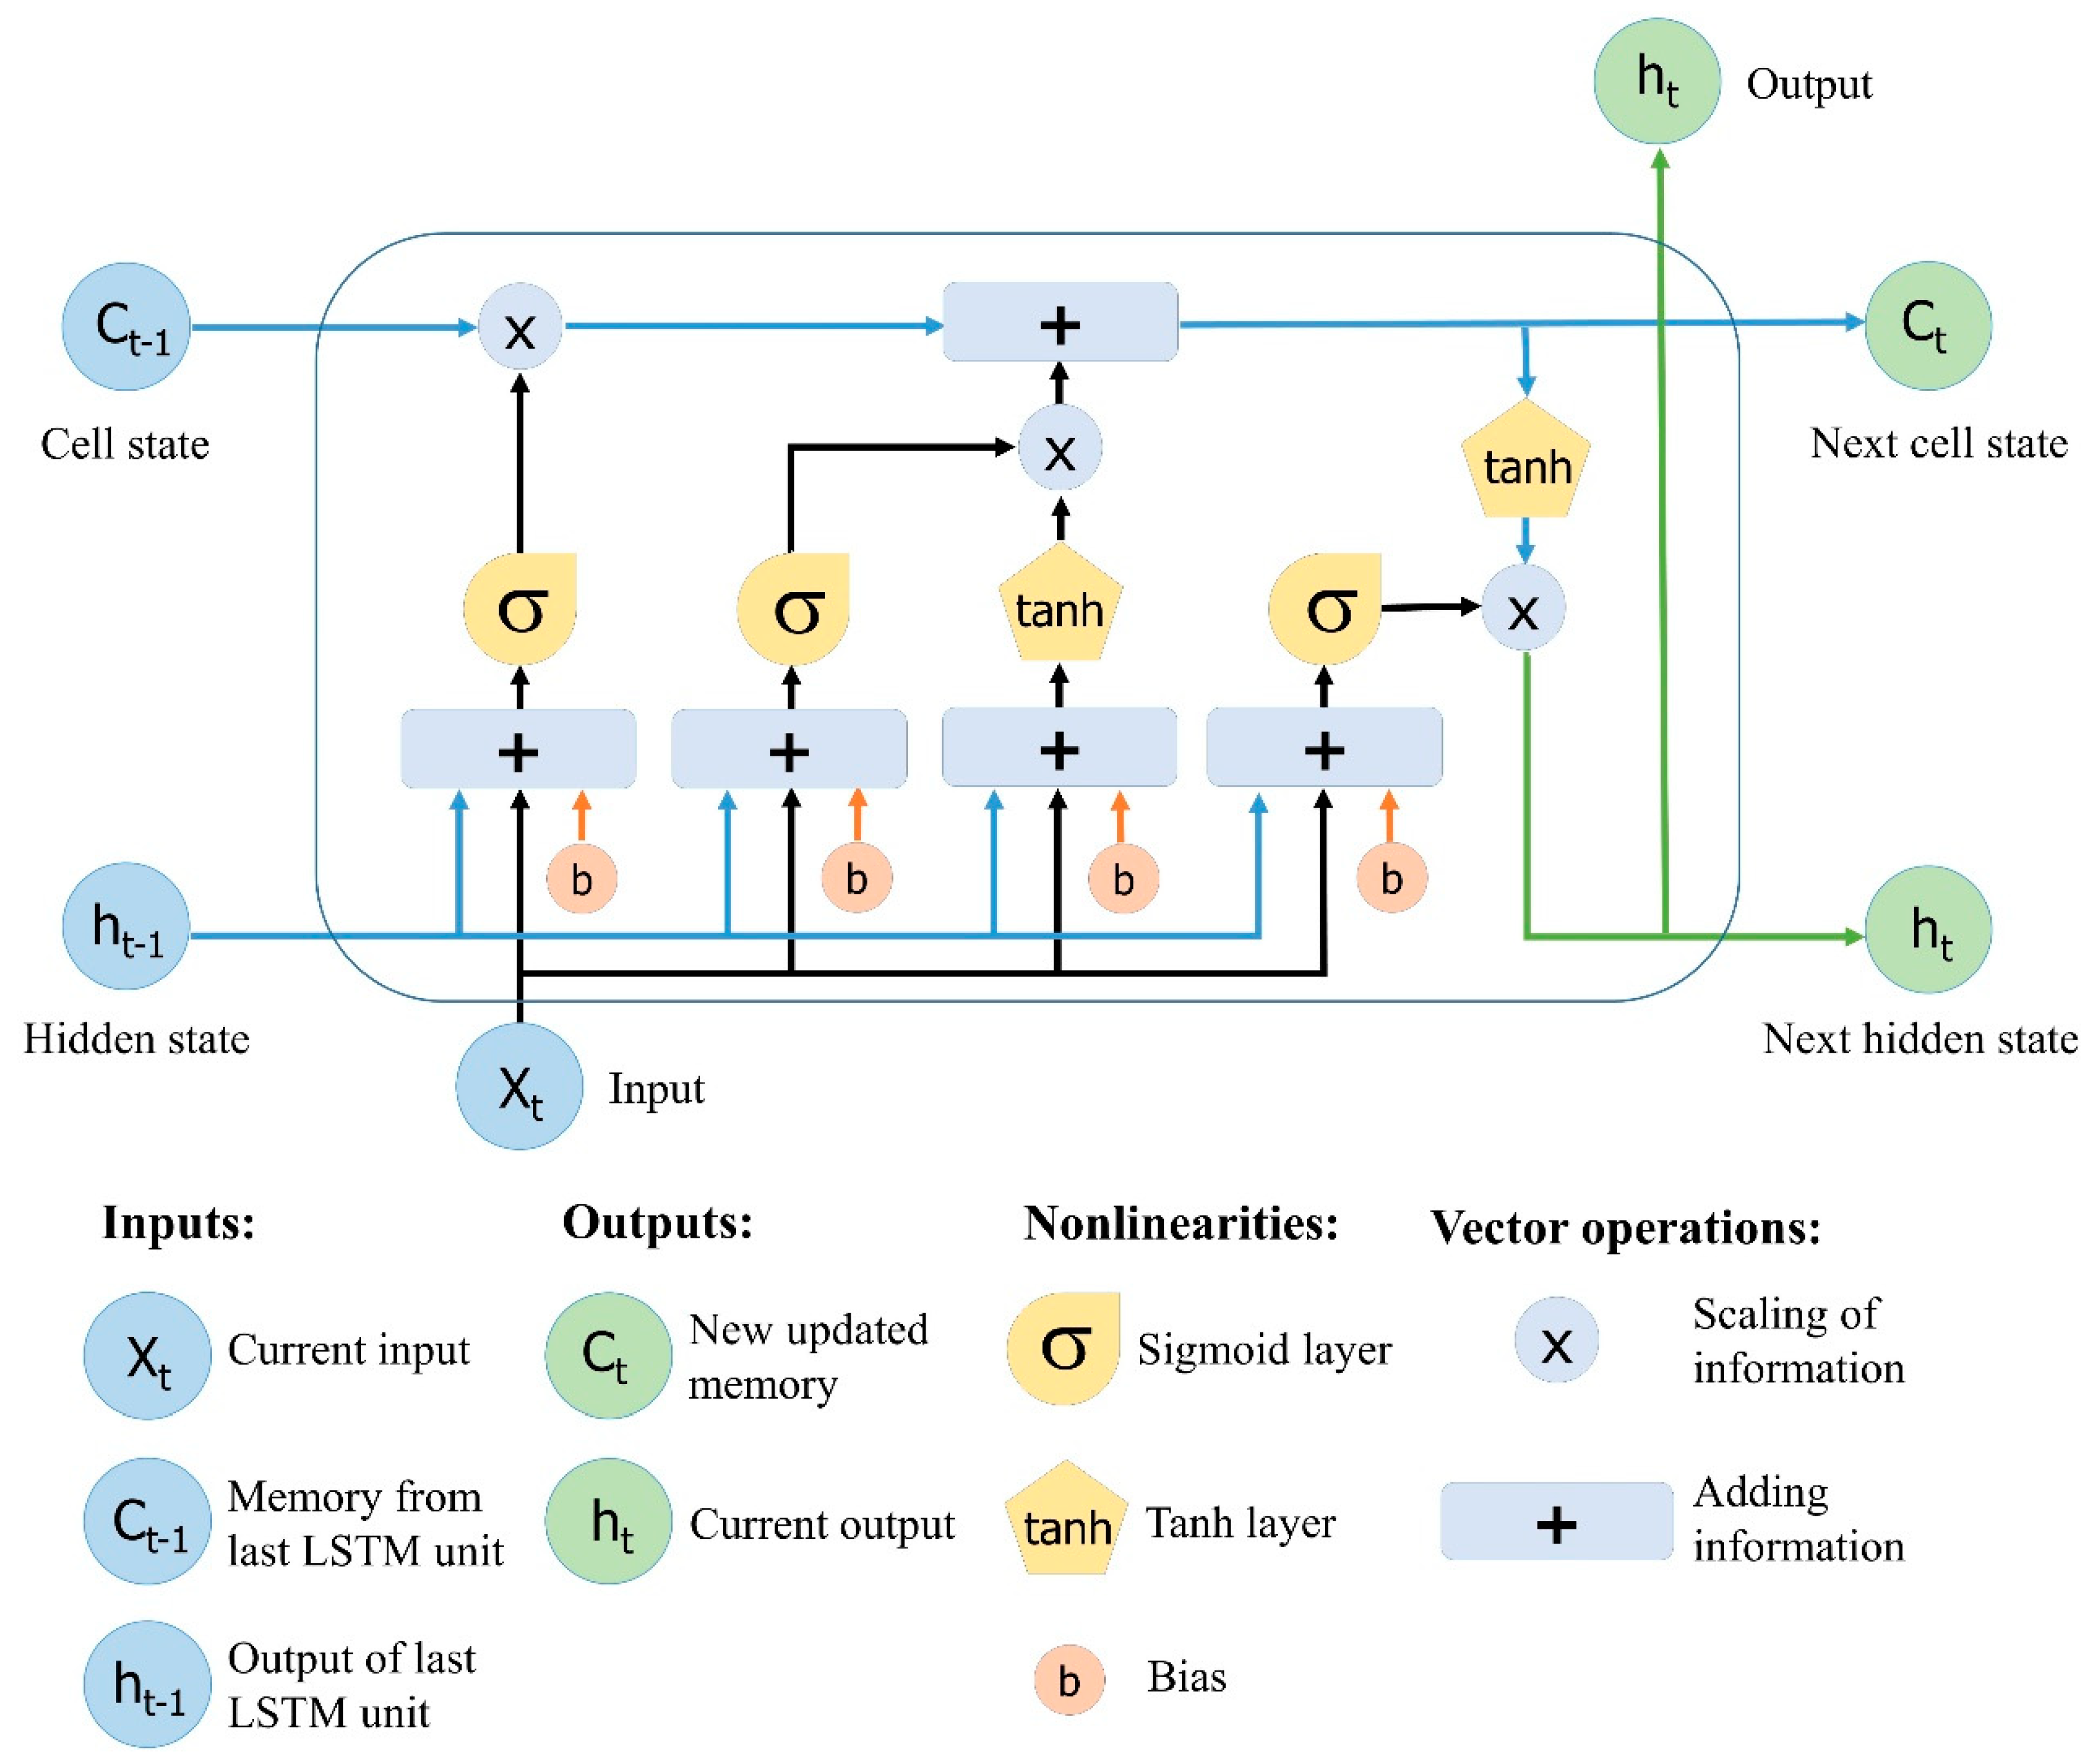
\includegraphics[scale=.55]{img/The_LSTM_cell.png} 
\caption{The Long Short-Term Memory (LSTM) cell can process data sequentially and keep its hidden state through time. image is taken from  \cite{}}
\label{fig:lstmcell}
\end{figure}

basic LSTM model consisted of two layers with  150 neurons in each layer, 0.2 dropout for regularization that drops nodes which prevent our model from overfitting, data is given in a batch size of 50 and 50 epochs.



\subsection{Pre-processing \&  Data preparation}
the training data was pre processed first to identify  outliers, a value was considered an outliers if it is 3 times greater than feature mean. we also add additional information in the form of  binary filter that indicates where missing that is, if a value is missing was marked 1.\\ 
Another way to mark missing data is the time delay between two consecutive non missing values.
Date is a a valuable data $Days\ ,Hours\ and\ Months$ can not be passed directly in their original form, that will be awfully misleading for our network since our network can not handle on its own the modulo operation. to prevent this problem  from happening we turn data into a cyclic data by decomposing it into pair of cosine and sine.
All these meta data will give additional information to train on.

As we are going train a large network, we would want to scale our data first between [0-1] in order to converge. and for that we transformed data between values 0 and 1 \cite{Chatterjee2017} using the \textbf{MinMaxScaler} function \ref{eq:MaxMin}.
%
\begin{equation}
\label{eq:MaxMin}
x_{scaled} = \frac{x_{i} - x_{min}}{x_{max} - x_{min}}
\end{equation}
%

\subsection{Output data preparation}
The LSTM was trained to predict 1 hour ahead, to do so we shift back our data to the last $look\ back$ sequences or time steps, it is important to remember that in order to predict sequence at time t+1 we " $look\ back$ "  at the last \in$ \left\{t,t-1,t-2,t-3...t-n\right\}$ with 'n = $look\ back$'  which is parameter to tune later in order to find the best value for it.


\subsection{Tensor Preparation for RNN input data}
Data sets is passed to the LSTM in a 3D tensor, where the first parameter is a batch dimension $n$, represents the number of observation we can process in parallel, the second parameter refers to the number of time steps or look back parameter that decide how many time steps we are going back to see in past in order to predict one sequence ahead in future, the third parameter is the number of features of our data set. for more illustration the figure below shows how data is feed into the LSTM network \ref{fig:tensor-tables} 
  
%
\begin{figure}[H]
\centering
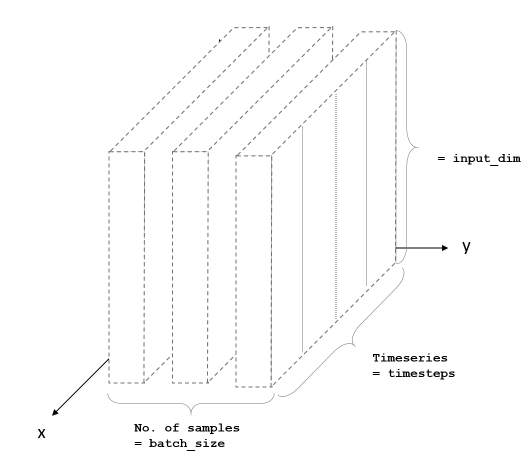
\includegraphics[scale=.45]{img/tensor.PNG}  
\caption{Process of converting data input columns into a Tensor for training the RNN \cite{tensor}.}
\label{fig:tensor-tables}
\end{figure}
%

\section{Results \& Expirements}

\subsection{Training \& Testing phase }
After pre-processing our data we were found with 11,508 samples. The organized data was split 80\% Train and 20\%  Test. Fitted  our data in  LSTM network \ref{fig:lstm-150} with total 123,751 trainable par5ameters.
%
\begin{figure}[H]
\centering
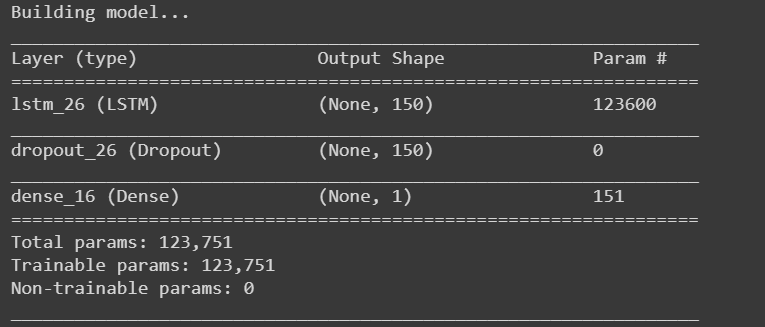
\includegraphics[width=.9\textwidth]{img/lstm_150.PNG}  
\caption{LSTM architecture with one layer}
\label{fig:lstm-150}
\end{figure}
%

we implemented an early callback to stop training before over-fitting if the loss value did not change after 2 epochs, a chart is showing the training set and test set loss during training this way we can monitor the training process.
In the figure below \ref{fig:verbose}, we can see that the test loss is lower than the training loss that is a good sign to  according to the evaluation model we saw in the previous chapter as we should always follow the bias-variace tradeoff \ref{}.

%
\begin{figure}[h]
\centering
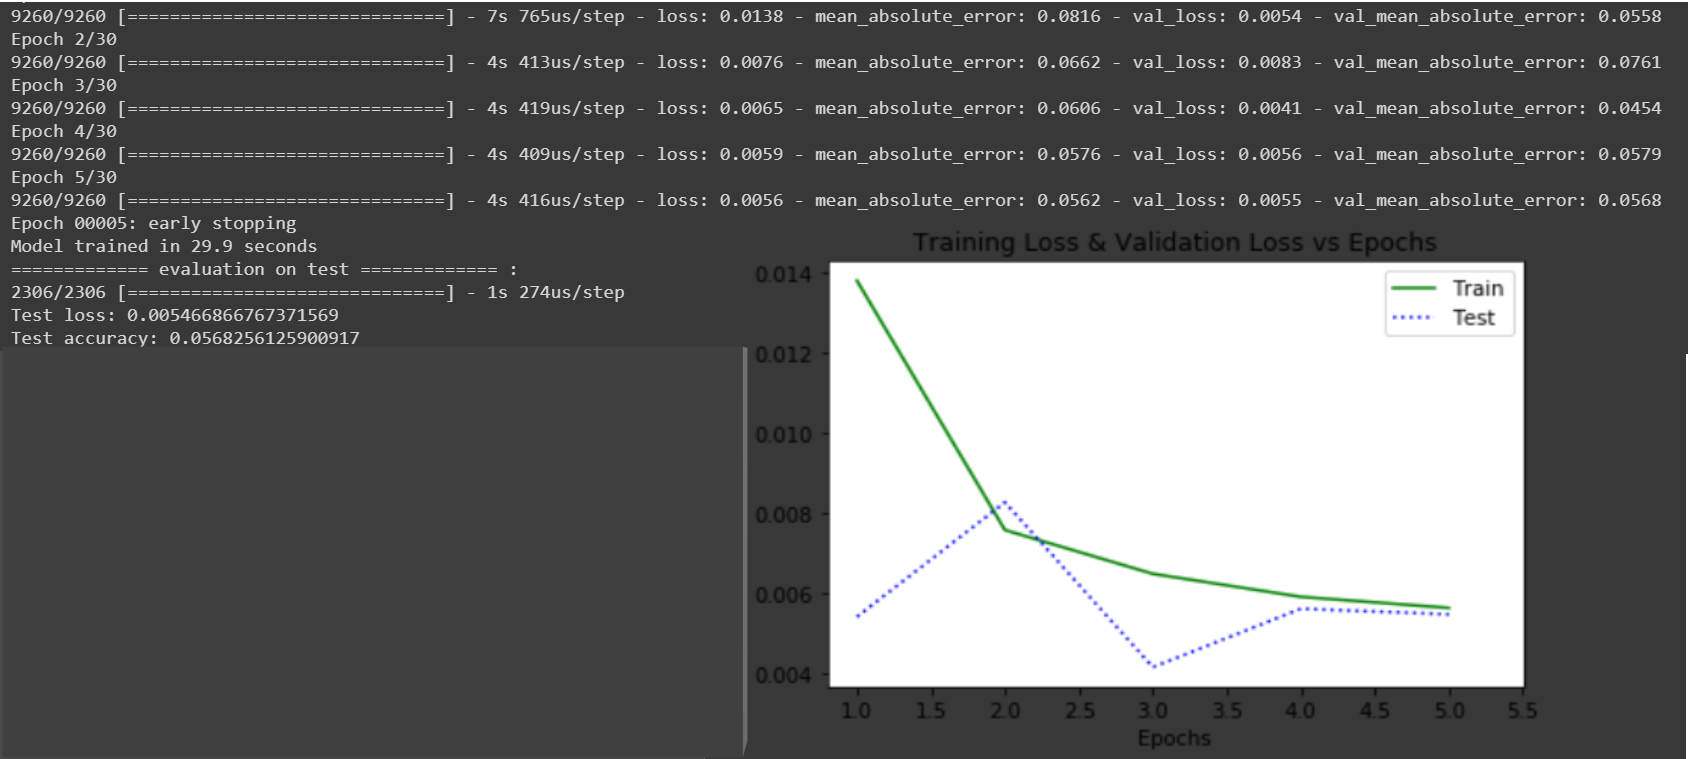
\includegraphics[scale=.4]{img/_verbose.PNG}  
\caption{cal loss}
\label{fig:verbose}
\end{figure}
%
The trained model is run on the test set which would then collect all predictions and calculate an error score. another metric was calculated for comparison; since RMSE is criticized for its over-biasing when measuring continuous variables.
\cite{Chai_Draxler_2014}.\\next step we can visualize how well our model can predict the target training data, 
%
\begin{figure}[h]
\centering
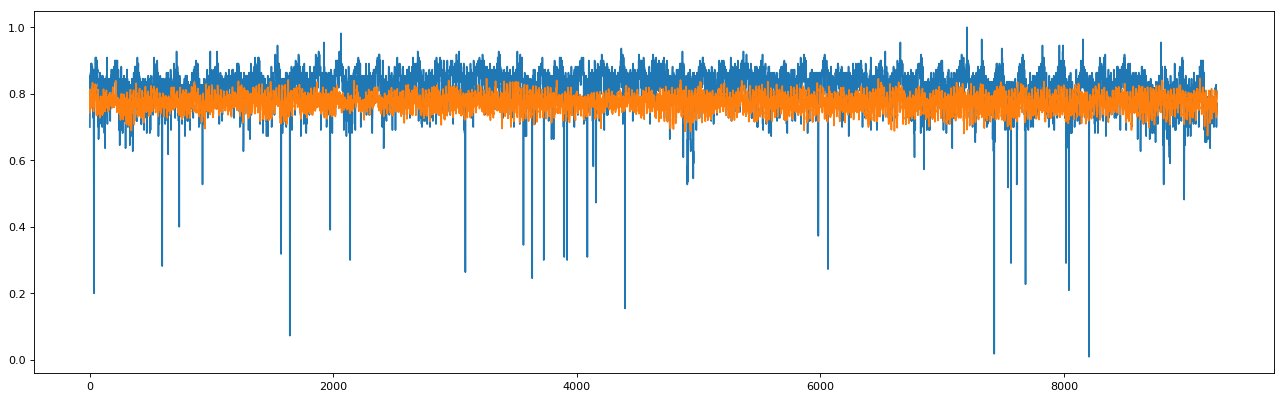
\includegraphics[scale=.4]{img/prevision_sur_training.png}  
\caption{prediction on training data set}
\label{fig:verbose}
\end{figure}
%
%
\begin{figure}[h]
\centering
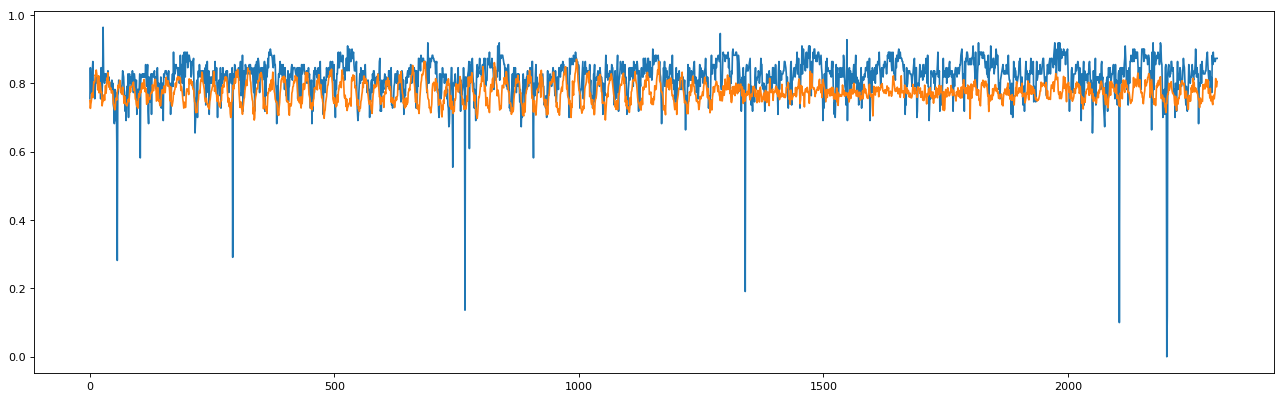
\includegraphics[scale=.4]{img/prevision_sur_test.png}  
\caption{prediction on testing  data set}
\label{fig:verbose}
\end{figure}
%
\newline
%
\begin{verbatim}
MAE : Train Score: 8.25  ,  Test Score: 7.94
RMSE : Train Score: 9.57  , Test Score: 9.62 
\end{verbatim}
%
As we can see from two figures of the prediction and the two  evaluations metrics (MAE and RMSE) we can judge that the first model with simple layer and 150 neurons, did eventually learn the seasonality and the pattern of data with an RMSE of 9.62 on testing data but still not enough to trust this model on imputing several missing hours. 

Note : one thing we should note, is that even though the MAE of training data is lower than testing data, which is normal in this case  since training data has 80\%  of original data whilst testing data is only 20\% of original data.

now we will test the model on imputation data set which has  several missing data 

\begin{figure}[h]
\centering
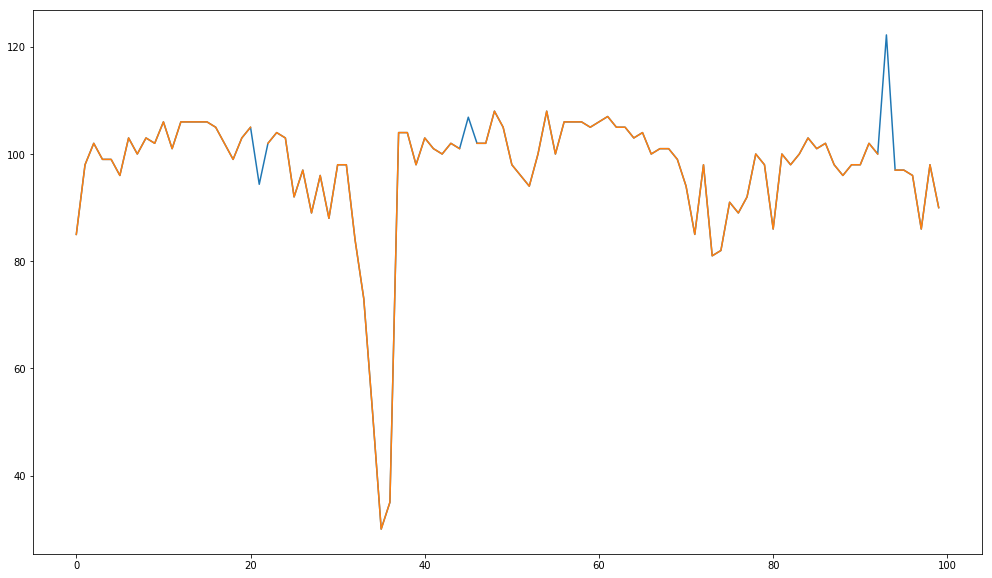
\includegraphics[scale=.32]{img/merge_best_of_result.png}  
\caption{the blue part is the imputation using  LSTM with one layer}
\label{fig:first_imp}
\end{figure}

the figure above\ref{fig:first_imp} shows the prediction of our model o the first 100 samples, and we can see that it can be in reasonable range when predicting 1h,2h. more than 3h it seems it starts to give unreasonable results, this is due to the accumulated error we have along with the prediction, in each prediction of t+1 we use the last L samples from past to impute the the future (t+1), but as in every machine learning or deep learning model the prediction always comes with an error (RMSE = 9.57). which means using the predicted values by the model to predict other future samples does have a really bad effect as we may see in the third Big gap in \ref{fig:first_imp}.

there is one way to solve this problem we suggest to increase the model complexity which will allow it to learn to generalize even better and minimize the error and for that we used another architecture  called  stateful stacked LSTM as the next figure will explain this new architecture :

\begin{figure}[h]
\centering
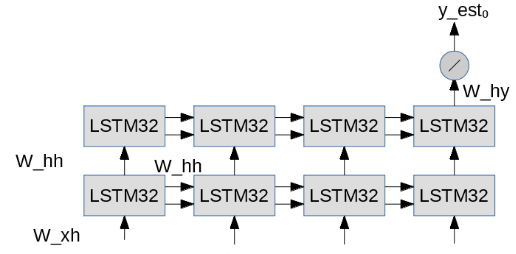
\includegraphics[width=0.55\textwidth]{img/stateful_stacked_lstm.png}  
\caption{stateful Lstm  architecture \cite{keras2015}}
\label{}
\end{figure}
we train the new model in the same data set as before and evaluate the error again using RMSE and MAE, we had the following results :
\begin{verbatim}
MAE : Train Score: 2.46  ,  Test Score: 2.09.
RMSE : Train Score: 1.94  , Test Score: 2.02 
\end{verbatim}
as we may notice that RMSE significantly dropped by using the stateful lstm architecture with different  number of neurons at each layer \ref{stat_lstm}. the training stopped at 20 epochs the val loss stopped improving.
\begin{figure}[!h]
\centering
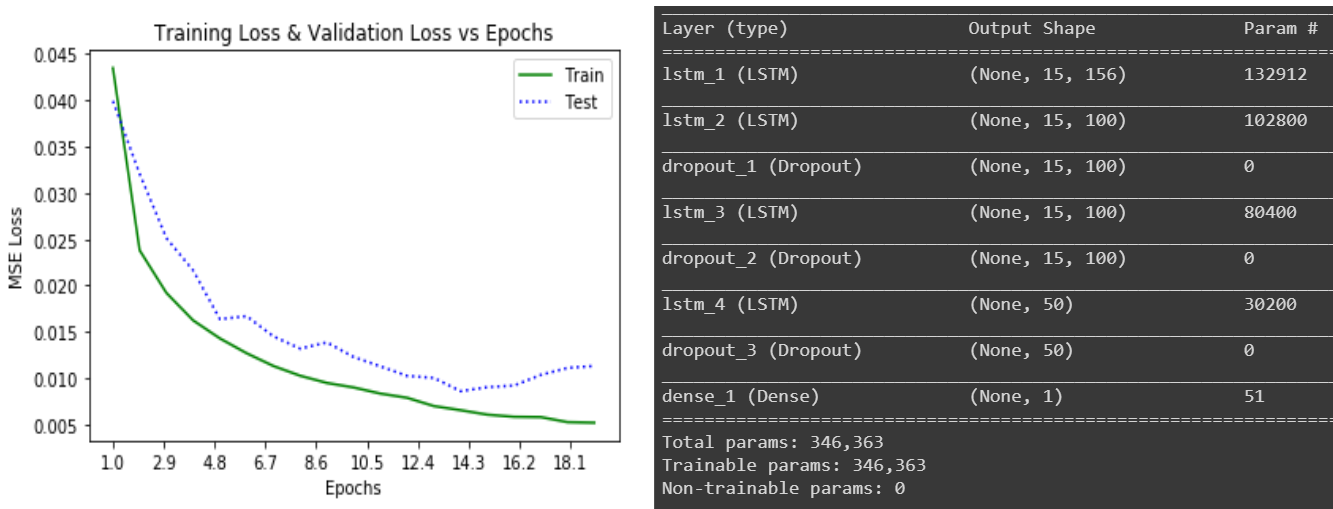
\includegraphics[width=1.05\textwidth]{img/lstm_stateful.png}  
\caption{The Stateful Lstm model and training loss vs validation Loss }
\label{stat_lstm}
\end{figure}
Now that we improved the accuracy of our model we can try and fit the model in order to estimate missing data, this time we will try it for even greater than 3h and see if it is within the possible range of the two Non missing values.
in the next figure we will visualize the first 500 of the original data that has a lot of missing data, as we can see it starts to give something really in the range.

\begin{figure}[!h]
\centering
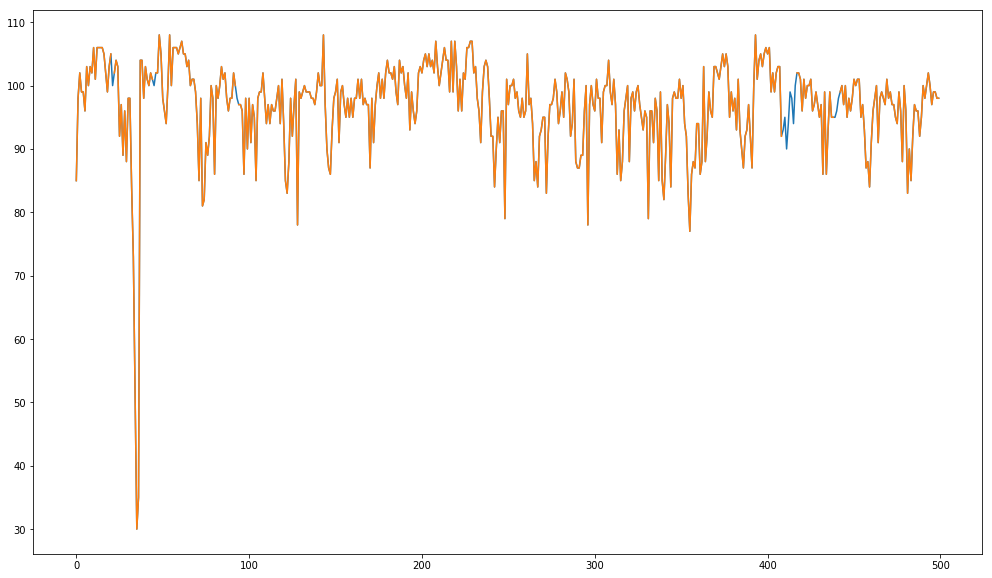
\includegraphics[scale=.4]{img/best_result.png}  
\caption{Testing the imputation}
\label{fig:verbose}
\end{figure}
the problem with our original data is that we can not quantify the error of Imputation phase, because we do not have Real values to compare our results to; in order to validate our model we would need a complete data.
we decide to  generate synthetic data, sprinkle randomly missing values or even gaps, and add features to mark the accumulated missing values, this  meta-data that indicates where the data is missing.\\the function used to  generate is $(-1)^{p}$ with $p \in N$,we trained our previous stateful model with the same parameters on 99988 samples, we let the output to be a probability, if we want perfect result we can turn the problem into binary classification with two possible outcomes -1 or +1; but we prefered to go with probability to see how it will be affected in longer gaps.
\newpage

The figure below confirms that Stateful stacked Lstm can  maintain even after 4h, with error prediction  of  0.9 in terms of RMSE, which is nearly perfect.    

\begin{figure}[!h]
\centering
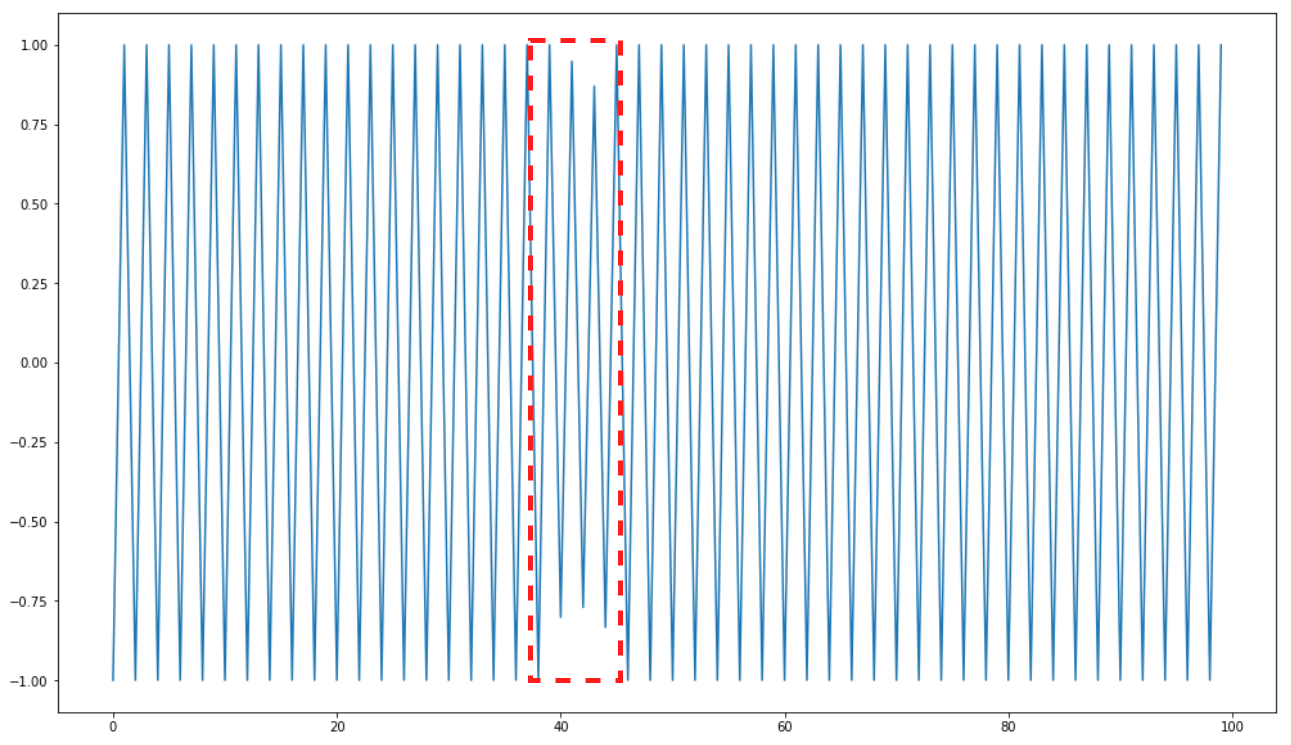
\includegraphics[scale=.4]{img/synthetic_data_lstm.png}  
\caption{Red part is the imputation of the stateful lstm }
\label{fig:state_lstm}
\end{figure}

stateful Lstm outperform all other models since it can model sequential data very good, can maintain information over time, can handle multiple variables, also can learn linear and non linear dependencies,it can  learn deep features in our data unlike ARIMA and other classical approaches.

\subsection{other tested models:}

In our experiments we tried other models as Time aware LSTM \cite{timeaware} which is a variant of  LSTM that try to inculde as input the time gaps made and based on the size of the gap we decide how  much the information flow from previous hidden states we are allowed to take in order to predict the next value ahead in the future.\\a more detailed and technical explanation of how T-Lstm work as authors  Baytas, Inci M.\cite{timeaware} explains : \say{Time Aware LSTM (T-LSTM) was designed to handle irregular elapsed times. T-LSTM is proposed to incorporate the elapsed time information into the standard LSTM architecture to be able to capture the temporal dynamics of sequential data with time irregularities. T-LSTM decomposes memory cell into short-term and long-term components, discounts the short-term memory content using a non-increasing function of the elapsed time, and then combines it with the long-term memory}.
unfortunately the T-Lstm failed to fit the training. and was not capable of learning the patterns nor imputing missing data.

another machine learning model we used and already mentioned in state of the art chapter is Adaboost(Adaptive Boosting) can be another good option for either Forecastign time series or even imputing data the only inconvenient we have is that it needs some kind of feature extractor from our time series we used tsfresh\cite{} which provide us with 100 feature to train our model with added to our original time series with One variable (as ARIMA).
to get around the " The Curse of dimensionality " we usually use some kind of dimensionality  reduction technics as PCA, SVD or Feature engineer to reduce number of features that can make time of calculations polynomial rather than exponential.

\begin{figure}[!h]
\centering
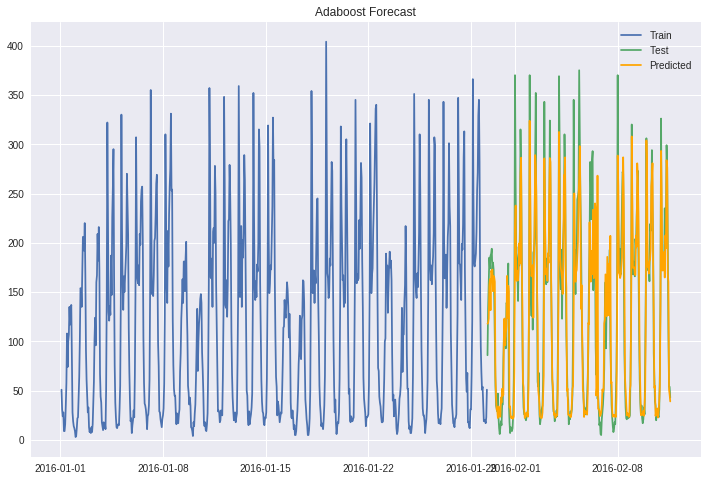
\includegraphics[scale=.6]{img/adaboost_results.png}  
\caption{Adaboost forecasting}
\label{fig:adaboost}
\end{figure}


\subsection{Transfer Learning}
Very much like one's ability to steer a car helps in learning to drive a motorcycle, the knowledge of a model contains by having been trained on one specific task might help in solving a related task.\\This is the general aim of transfer learning: to transfer knowledge from an already trained model to a different domain or a different task.\\ in our use case Transfer learning was never used before to impute missing data for a damaged sensor, it is still a low researched field. Nevertheless, to solve some issues as stated in first section of this chapter \ref{contextofimp}. our proposed solution is to use transfer learning of The nearest Neighbor of the damaged sensor that respect a number of  criterion  such as measuring the same physical property (temperature, humidity...),
being at the same height, and spatially correlated.
having trained LSTM for each sensor, we can easily transfer learning of one sensor into another damaged sensor in order to impute in real time.\\ All in all, domain adaptation for IOT sensors, is a fresh idea and needs a lot of experiments on the field. However the idea is already working in a number of fields as "style transfer" for images and art \cite{transferlearning}, NLP openAI released their GPT-2 which made it possible for people to use transfer learning to customize their models, more on this subject on \cite{nlp},   



\section{Conclusion}
the reccurent neural networks are good for modeling sequential data whether it is in text data, or Time series, other variants or RNN can be tested also such as  Gated Recurrent Network, which is a variant of the LSTM. There is also the Attention Network that considered now the state of the art in NLP field, which is also a variant of LSTM. and Bidirectional LSTM means allowing information to flow not only from left to right but also of from right to left, the two sides are concatenated, and then make predictions. 




% \section{Acknowledgments}

\chapter{Discussion and Recommendations} \label{hgr}

\section{Discussion  }

In this work, we performed a benchmarking of statistical methods and deep learning predictive  models, we showed that most of models fail to perform well on imputation task. However, they perform very well in other areas of artificial intelligence.

ARIMA has a good predictive effect on short-term forecasts, while LSTM has a good predictive effect on long-term models. to summarize Arima's way to deal with sequential data, focuses on univariate data with linear relationships and fixed lag  diagnostic time dependence,also studying the correlation between observations at different times, which requires analysis and interpretation of the number of lag observations. therefore it is suitable to use ARIMA  when we have to deal with small datasets, from our experimentation we found that arima performance decrease when working with a large data sets. On the other hand, Recurrent Neural Network especially LSTM seems to be more suitable for large datasets. Mainly this is due to  the fact that deep learning  provide a way to divide data  into smaller batches and train them in multiple stages allow the network to learn deep features,and able to lean temporal dependencies from context by observing the sequence from a certain time, additionally lstm  can model complex multivariate sequences.\\LSTM is undoubtedly more complex and difficult to train, and in most cases its performance will  exceed the performance of a simple ARIMA model.\\Machine learning and deep learning methods have not yet fulfilled their promise of univariate time series prediction, and there is still much to be done in this area.


\section{Recommendations}
First thing in order to impute missing data, we should always know and understand the context of how the data was missing, asking a question as:  was there any data to receive ?, meaning if the data is missing because of the lack of any information, there is no use to impute this data, the second question we should usually ask is what missing mechanism we are dealing with, missing data always introduce bias but there are Mechanism that are way less biased than others, thus, the importance of recognizing the mechanism of missingness we are dealing with as already explain in data mechanism section MCAR or Missing Completely At Random, is the only mechanism that we are allowed to  use List-wise deletion which is dropping rows with missing data.However in real life problem it is really hard to prove that your data is missingness pattern is stochastic (MCAR) , theoretically it is not possible to prove, Most of the time we are dealing with MAR and MNAR.\\The imputation technics that you can use depends on ur missingness regime and also nature of your data if it is sequential data as our project then usually you will have to work with models that can model time series such as ARIMA, SARIMA,RNN...etc. But using the mean imputation can be a total destruction for your results and over biasing your parameters model.

\section{perspectives and future works }

Stateful Stacked LSTM outperforms all simple lstm and Arima along with others tested models this is a good solution for imputation missing data from past, But what we hope to develop in the future is using future information to impute missing data as we can see in figure \ref{fig:extrapo}  we usually know the non missing values on the end of each gap they are marked with blues in figure below.so extrapolation rather than interpolating seems promising for our future development, However there is a variant called Bidirectional Recurrent neural network, and the idea behind it is using both future information and past information  to predict an event that happened between the past and the future,some researcher as Cao, Wei, \cite{brits} used this architecture to impute missing. 

\begin{figure}[H]
\centering
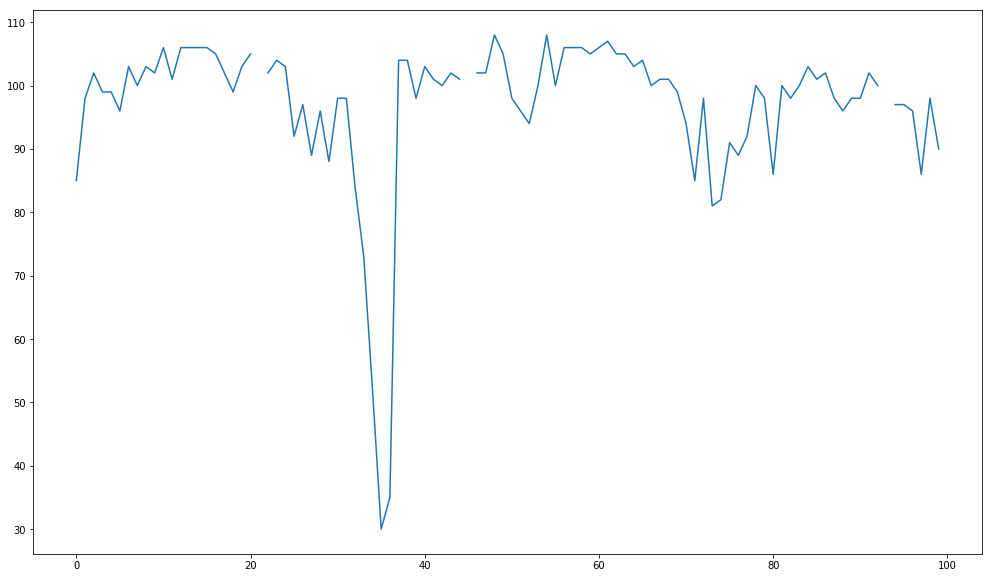
\includegraphics[width=0.6\textwidth]{img/extrapoalting.png}
\caption{the two ending non missing values of a gap}
\label{fig:extrapo}
\end{figure}

Yet another type of architecture we did not study in this project is Non-Autoregressive, since  autoregressive models  suffer from error propagation which becomes catastrophic for imputing long-range sequences, instead we can use  deep generative models. as in the following paper that was published on may 2019 under the name NAOMI: Non-Autoregressive Multiresolution
Sequence Imputation. \cite{naomi}.




\section{Acknowldgement}

We'd like to express our gratitude to our supervisor, Bertand Leger, for his guidance  throughout our research and shared with us his vast knowledge and
experience in the fields of internet of things and machine learning.

Also i would like to thank   '' la Direction Interdépartementale des Routes Est (DIR Est) for giving us access to their traffic database which. 



%\chapter*{Conclusion and Perspective}






In this work, we succeed in building an HGR system that is able to detect the presence of two hands, to recognize the meanings of a gesture  in a predefined vocabulary. and The lighting conditions, signers skin colours and clothing, and background  have little impact on the performance of this HGR system. 
In this project we used Microsoft kinect for data acquisition of depth images. At  First we were focusing on giving the user a better experience by tracking and  detecting the hand  in a range of [80cm , 3 meters]  allowing the  user to move freely around the camera. then we extract features using two powerful descriptors SIFT(Scale Invariant Features Transform) and SURF(Speeded Up Robust Features) a  third descriptor(Fourier shape descriptor)  was added to complete the requirement of a robust HGR system. having our stable keypoints that are invariant to scale and rotation  we used machine learning algorithms SVM, K-means and Nearest Neighbors  to classify our  16 gestures. afterwards we generate a codebook based on the keypoint of sift and surf,we also did  a comparative study between sift and surf performance's based on their generalization performance, Finally we conclude that surf outperform sift with an Average AUC of 98\% with RBF kernel against 91\% for sift, the only problem with these two descriptors is that they are computationally expensive which blocks their application on rela time applications,Hence the need for a fast descriptor such as fourier descriptor.

\begin{itemize}
    \item this application can detect  in a minimum range of 80 cm and maximum range of 2 and half meters until 3 meters.
    \item The application is optimized and make no calculation or classification if there is no \textbf{Human body} in front of the camera, the program starts only when u make a gesture to recognize the human skeleton.
    \item A powerful CPU or  GPU can make  sift and surf descriptors along with BOF algorithm to work fine especially with the recent implementations of OpenCV for SURF GPU and SIFT GPU.
    \item the project is extendable in term of adding any new gestures to the vocabularies (as long as  they have a different shape).
    \item Kinect Version 1 (used for this project) gives limited depth range of 3 meters (theoretically 4 meters),and gives false hands positions  especially if the hands cross. he error increases respectively with depth.  To the author  best knowledge the Kinect version 2 gives more depth range until 8 meters and uses good filters for to stabilize body joints positions. 
    \item the hands images taken by the camera were only of an individual person, which is the author of this project, this can probably causes our application to overfit a little bit, but this problem can be easily solved with if we shoot with  the different persons with different shape of hands and to account for the different ways that people might perform those gestures.this will help a lot in boosting the generalization performance of our application.
   
\end{itemize}


This project was an opportunity to apply the different knowledge acquired during our studies in the IST master; especially as we have deepened our knowledge in the field of computer vision by applying image processing techniques using the OPENCV library. We also learned new skills at programming with the Kinect SDK. Moreover; this work allowed us to master some of Machine learning aspects as well as learning the necessary steps to have a good performance of generalization.


Our application performs the recognition of the static gestures of the both  hands. Thereby It is very important to deepen this work by recognizing the gestures dynamically in order to establish a system that is able to translate the sign language into a natural language and include Text To Speech (TTS) protocol. 





\appendix
%

\chapter{How is Missing data is biasing ?}

\section{Introduction}\label{sec:kinect}



\subsection{Working  Environment  Introduction }
The system of the present project  consists of three main components:  Hand Detection, preprocessing ,  Gesture Recognition.  This system is built upon  The \textbf{Kinect SDK}  framework the was  used to extract  depth data  from the Kinect sensor.\textbf{C++} was chosen as the main language for this project for its efficient speed and the least memory usage  there is also \textbf{Python} that was used for  evaluating tasks and measure accuracy.


\subsection{Kinect's Features }

Hardware The Kinect has one RGB camera, one depth sensor that consist of one Infra-Red (IR) projector and one IR camera, an array of four microphones and a motorized tilt for changing the field of view \cite{kinect15}. These components are shown in \ref{fig:cam2}

\begin{figure}[H]
\centering
\includegraphics[width=0.53\textwidth]{img/kinectcamera2.png}
\caption{ kinect Hardware }
\label{fig:cam2}
\end{figure}

\textbf{The RGB sensor}  (or video camera) provides 2D view of the scene in three basic colors: Red,Green, and Blue \cite{kinect15} The resolution that can be used is 640x480 pixels or 1280x960 pixels with 32 bits per pixel and the frame rate of 30 frames per second (fps) \cite{kinect15}. \\

\textbf{The depth sensor} \\
– the IR Projector is used to illuminates the scene with structured light while the IR camera observes this illuminated scene and measures the distance of objects from Kinect \cite{kinect15}. As result a depth map is created that gives the distance of objects from the sensor. The depth
map resolution is provided in 320x240 pixels or 640x480 pixels with 16 bits per pixel and an  output frame rate of 30fps \cite{kinect15}. The minimum depth sensor range is from 0.8 meters to a maximum of 4 meters (physical limits). The recommended distance (“Sweet spot” in figure 2.6) is between 1.2m and 3.5m and distances beyond 4m are not recommended since noise get larger \cite{kinect17}. Sun light interferes with infrared light, therefore the depth sensor is not well suited for applications in direct sun light conditions (outdoors)\cite{kinect17} .  

\begin{figure}[H]
\centering
\includegraphics[width=0.8\textwidth]{img/afterworking1.png}
\caption{Kinect depth sensor capabilities}
\label{fig:cam3}
\end{figure}

`\textbf{The motorized tilt}\\
 is used to control the field of view as shown in figure \ref{fig:cam4} and it characteristics are \cite{kinect15} : 
 
\begin{itemize}
\item  Horizontal field of view: 57.5 degree,
\item  Vertical field of view: 43.5 degree,
\item Tilt range: -27 to +27 degree range up and down.

\end{itemize}

\begin{figure}[H]
\centering
\includegraphics[width=0.6\textwidth]{img/afterworking2.png}
\caption{Kinect depth sensor capabilities}
\label{fig:cam4}
\end{figure}

\textbf{The microphone array} \\
is used for capturing sounds and usually used for speech recognition. It consist of four microphones that enable detection of sound’s source and direction of audio wave \cite{kinect15}. One of them is located at the left of IR projector and the other three microphones are evenly spaced and located at the right of IR camera as shown in \ref{fig:cam5}. The sensor can detect sounds in range of -/+ 50 degree in front of it (\ref{fig:cam5}.a), sound direction in 10 increments  (\ref{fig:cam5}.b) , and offers 20dB (decibel) ambient noise cancellation (\ref{fig:cam5}.c)\cite{kinect17}.

\begin{figure}[H]
\centering
\includegraphics[width=0.8\textwidth]{img/afterworking3.png}
\caption{Kinect sound sensor capabilities a) audio range detection b) sound direction localization c) ambient noise cancellation .
}
\label{fig:cam5}
\end{figure}


\textbf{Skeletal tracking }\\
Skeletal tracking is offered through depth camera. Up to six people can be tracked, while the full skeleton is provided only for two. In full skeleton tracking mode, 20 joints are tracked while in seated mode, half of them (10 joints).The accuracy is larger when the user stands in front of the Kinect, while side standing poses some challenges. Skeletal tracking and two modes are  illustrated in \ref{fig:cam6}.

\begin{figure}[H]
\centering
\includegraphics[width=1.0\textwidth]{img/afterworking4.png}
\caption{Skeleton tracking modes through Kinect }
\label{fig:cam6}
\end{figure}

The tracked joint positions are shown in \ref{fig:cam77}
\begin{figure}[H]
\centering
\includegraphics[width=0.4555\textwidth]{img/afterworking5.png}
\caption{Skeleton joint positions offered  through Kinect }
\label{fig:cam77}
\end{figure}

Each skeleton position (body center) and each joint is provided in 3D (x, y, z) coordinates as 
shown in \ref{fig:cam7}. The Kinect is placed at the origin of coordinative system and from Kinect viewpoint: positive Z-axis increases towards the user, positive  Y-axis increases upward and positive  X-axis increases to the left .  

\begin{figure}[H]
\centering
\includegraphics[width=0.7\textwidth]{img/afterworking6.png}
\caption{kinect skeleton coordinate system  }
\label{fig:cam7}
\end{figure}


 
\subsection{linking  kinect SDK with visual studio}

We are using the Kinect SDK version 1.8 and this is how the project is configured. Please note that the developer machine is Windows 7 x86. 
If you are using x64, please change the path accordingly.\\
\textbf{Step 1. } In the Property Manager, right click on the project name and select Add New Project Property\\
Copy C:/Program Files/MicrosoftSDKs/Kinect/v1.0/inc\\
Copy C:/Program Files/MicrosoftSDKs/Kinect/v1.0/lib (you will have both x86 and x64 libraries)\\
\textbf{Step 2}. Configure the project. \\
C/C++ -$>$ General-$>$ add C:/Program Files/Microsoft SDKs/Kinect/v1.8/inc to your Additional Include Directories\\
Linker -$>$ General -$>$ add" C:/Program Files/Microsoft SDKs/Kinect/v1.8/lib/amd64 "  to your Additional Library Directories (if you are configuring for x64, use the amd64 directory)\\
Linker -$>$ Input -$>$ add "Kinect10.lib" to Additional Dependencies\\
\textbf{Step 3}. Compile\\

%
\chapter{Opencv}

\section{Introduction }
OpenCV (Open Source Computer Vision Library) is released under a BSD license and hence it’s free for both academic and commercial use. It has C++, C, Python and Java interfaces and supports Windows, Linux, Mac OS, iOS and Android. OpenCV was designed for computational efficiency and with a strong focus on real-time applications. Written in optimized C/C++, the library can take advantage of multi-core processing. Enabled with OpenCL, it can take advantage of the hardware acceleration of the underlying heterogeneous compute platform. 
\subsection{Build and install Opencv with Opencv Contrib}

\begin{enumerate}
\item Download CMAKE.
 \url{https://cmake.org/download/}
\item Install Visual studio 2017 Community, with C++ and C support.
\item download Opencv 3.2.0 and opencv\_contrib-3.2.0.
\item launch CMake application and then specify the source and build directory as shown in figure below. The red box must be filled with the directory path of OpenCV source, and the green box must be filled with the directory path of designated build folder.

\begin{figure}[H]
\centering
\includegraphics[width=0.9\textwidth]{img/working1.png}
\caption{ setting Cmake right directories }
\label{fig:working1}
\end{figure}

\item we can hit several times  configure. Until we have some list of possible settings like on image below. Use different settings and configuration options. choose  solution we want. FFMPEG, OPENCL support and \textbf{generate OPENCV.SLN file inside  opencv3.0 build folder.} 

\begin{figure}[H]
\centering
\includegraphics[width=0.9\textwidth]{img/working2.png}
\caption{ result after building }
\label{fig:working2}
\end{figure}

\item FIRST just select DEBUG, x64 version like on picture, click right mouse on Entire solution and hit BUILD  . 

\item 	Second you need to switch from DEBUG to RELEASE and build the solution again. \textbf{This build} also Cmake target install, (you can see this under install) where  your installation is located. \\
Your installation location usually is under opencv32build/install .

\end{enumerate}

\subsection{linking Visual studio with opencv :}

\begin{enumerate}
\item OpenCV visual studio and create a console application 
\item in configuration Properties -$> C/C++ $-$>$ Additional Include Directories , then add OpenCV's Includes folders :
 \begin{itemize}
     \item C:/opencv/build/include
     \item C:/opencv/build/include/opencv
     \item C:/opencv/build/include/opencv2
   \end{itemize}
\item in configuration Properties -$>Linker$-$>$Additional Library Directories -$> $ add folder lib of OpenCV :\\
     C:/opencv/build/x64/vc14/lib 
\item in configuration Properties$->$ Linker$->$Additional Dependence$->$ add folder lib of OpenCV .
 \begin{itemize}
     \item opencv\_world320d.lib
     \item opencv\_features2d320d.lib
     \item opencv\_xfeatures2d320d.lib
   \end{itemize}

\end{enumerate}





%%%%%%%%%%%%%%%%%%%%%%%%%%%%%%%%%%%%%%%%%%%%%%%%%%%%%%%%%%%%%%%%%%%%%%%%%%%%%%%%%%%%%%%%%%%%%%%%%%%%%%%%%
\medskip



\begin{thebibliography}{80}



\bibitem{dempetrubin}
Dempster A.P. and Rubin D.B. (1983) Introduction pp.3-10, in Incomplete Data in Sample Surveys (vol. 2): Theory and Bibliography (W.G. Madow, I. Olkin and D.B. Rubin eds.) New York: Academic Press.)rld Federation of the Deaf. Retrieved 17 August 2013.
 
 \bibitem{rubin}
 Rubin, D. B. (1976). Inference and Missing Data. Biometrika, 63, 581-590. 

 \bibitem{nadam} Dozat, Timothy. "Incorporating nesterov momentum into adam." (2016).
 
 \bibitem{timeaware}
 Baytas, Inci M., et al. "Patient subtyping via time-aware LSTM networks." Proceedings of the 23rd ACM SIGKDD international conference on knowledge discovery and data mining. ACM, 2017.
 
 \bibitem{brits}
 Cao, Wei, et al. "BRITS: bidirectional recurrent imputation for time series." Advances in Neural Information Processing Systems. 2018.
 
 \bibitem{naomi}
 Liu, Yukai, et al. "NAOMI: Non-Autoregressive Multiresolution Sequence Imputation." arXiv preprint arXiv:1901.10946 (2019).
 
 \bibitem{Little2002}
 Little, Roderick JA, and Donald B. Rubin. Statistical analysis with missing data. Vol. 793. John Wiley & Sons, 2019.
 
 \bibitem{Chai_Draxler_2014}
 Chai, Tianfeng, and Roland R. Draxler. "Root mean square error (RMSE) or mean absolute error (MAE)?–Arguments against avoiding RMSE in the literature." Geoscientific model development 7.3 (2014): 1247-1250.
 
 \bibitem{tensor}
 https://medium.com/@shivajbd/understanding-input-and-output-shape-in-lstm-keras-c501ee95c65e
 
 \bibitem{listwise}
 King, G., Honaker, J., Joseph, A. and Scheve, K., 1998, July. List-wise deletion is evil: what to do about missing data in political science. In Annual Meeting of the American Political Science Association, Boston.

\bibitem{singleimp}
Kim JO, Curry J. The treatment of missing data in multivariate
analysis. Sociol Methods Res 1977; 6: 215-41.

\bibitem{mean}
 Malhotra N. Analyzing marketing research data with incomplete information on the dependent variable. J Mark Res 1987; 24: 74-84.
 
 \bibitem{Hastings1947}
 Hastings, C., Mosteller, F., Tukey, J.W. and Winsor, C.P., 1947. Low moments for small samples: a comparative study of order statistics. The Annals of Mathematical Statistics, 18(3), pp.413-426.
 \bibitem{brockwell2006introduction}
 Brockwell, Peter J., and Richard A. Davis. Introduction to time series and forecasting. springer, 2016.
 \bibitem{tong1990non}
 Tong, Howell. Non-linear time series: a dynamical system approach. Oxford University Press, 1990.
 \bibitem{box2015time}
 Box GE, Jenkins GM, Reinsel GC, Ljung GM. Time series analysis: forecasting and control. John Wiley & Sons; 2015 May 29.
 
 \bibitem{adaboost}
 Freund, Yoav, and Robert E. Schapire. "Experiments with a new boosting algorithm." icml. Vol. 96. 1996.
 
 \bibitem{hist_rnn}
 Hecht-Nielsen, R., 1992. Theory of the backpropagation neural network. In Neural networks for perception (pp. 65-93). Academic Press.
 
 \bibitem{Graves2013a}
 Graves, A., 2013. Generating sequences with recurrent neural networks. arXiv preprint arXiv:1308.0850.
 
 \bibitem{DBLP:journals/corr/Lipton15}
 Lipton, Zachary C., John Berkowitz, and Charles Elkan. "A critical review of recurrent neural networks for sequence learning." arXiv preprint arXiv:1506.00019 (2015).
 
 \bibitem{keras2015}
  author= {Chollet, Fran\c{c}ois and others},title= {Keras: Deep Learning library for {T}heano and {T}ensorFlow}, how published = {github.com/fchollet/keras},year= {2015}, note = {http://github.com/fchollet/keras},
  publisher    = {GitHub}, timestamp    = {2017-05-19}, url={http://github.com/fchollet/keras}
  
  \bibitem{nlp}
  http://ruder.io/state-of-transfer-learning-in-nlp/
  \bibitem{transferlearning}
  Jing, Y., Yang, Y., Feng, Z., Ye, J., Yu, Y. and Song, M., 2019. Neural style transfer: A review. IEEE transactions on visualization and computer graphics.
  
\end{thebibliography}



\end{document}
